\documentclass[xcolor={dvipsnames}]{beamer}

\usepackage{amsmath}
\usepackage{amsthm}
\usepackage[T1]{fontenc}
\usepackage[utf8]{inputenc}
\usepackage{MnSymbol}
\usepackage{stmaryrd}
\usepackage{upquote}
\usepackage{bussproofs, semantic, framed}
\usepackage{array}
\usepackage{hyperref}
%\usepackage{hanging}

\usepackage{graphicx}
\usepackage{cellspace}
\setlength\cellspacetoplimit{4pt}
\setlength\cellspacebottomlimit{4pt}
% for showing frames while development
%\usepackage{showframe}
\usepackage{caption, subcaption, wrapfig}
\usepackage{textcomp, scrextend}
%\usepackage{xcolor}
\usepackage[english]{babel}
\usepackage{url}
\usepackage{setspace}
\usepackage{esint}
% \usepackage{natbib}
\usepackage[backend=bibtex,
            style = numeric-comp,
            sorting = none,
            natbib = true,
            doi = false,
            isbn = false,
            url = false,
            %location = false,
            %publisher = false,
            hyperref = true]{biblatex}

\definecolor{ltblue}{rgb}{0,0.4,0.4}
\definecolor{dkblue}{rgb}{0,0.1,0.6}
\definecolor{dkgreen}{rgb}{0,0.4,0}
\definecolor{dkviolet}{rgb}{0.3,0,0.5}
\definecolor{dkred}{rgb}{0.5,0,0}
\definecolor{battleshipgrey}{rgb}{0.52, 0.52, 0.51}

\usepackage{listings}

\usepackage{defense-slides/haskell}
\usepackage{cmll}
\usepackage{pdflscape}

\usepackage{tikz}
\usepackage{tikz-qtree}
%\usetikzlibrary{arrows.meta}

\usepackage{parskip}
\usepackage{xspace}

\usepackage[style=british]{csquotes}

\def\signed #1{{\leavevmode\unskip\nobreak\hfil\penalty50\hskip2em
  \hbox{}\nobreak\hfil--- #1%
  \parfillskip=0pt \finalhyphendemerits=0 \endgraf}}

\newsavebox\mybox
\newenvironment{aquote}[1]
  {\savebox\mybox{#1}\begin{quote}}
  {\signed{\usebox\mybox}\end{quote}}


% \usepackage[capitalize, nameinlink]{cleveref}
% \crefformat{section}{\S#2#1#3} % see manual of cleveref, section 8.2.1
% \crefformat{subsection}{\S#2#1#3}
% \crefformat{subsubsection}{\S#2#1#3}

% \newcommand\fnurl[2]{%
%   \href{#2}{#1}\footnote{\url{#2}}%
% }
\mode<presentation>{\usetheme{Madrid}}


\newcommand{\tightoverset}[2]{%
  \mathop{#2}\limits^{\vbox to -.5ex{\kern-0.75ex\hbox{$#1$}\vss}}}

\newcommand{\BI}{\textbf{\em BI}\xspace}
\newcommand{\HM}{\textbf{\em HM}\xspace}
\newcommand\sepimp{\mathrel{-\mkern-6mu*}}
\newcommand\shimp{\twoheadrightarrow}

\newcommand{\M}{\mathcal{M}}
\newcommand{\W}{\mathcal{W}}
\newcommand{\Unf}{\mathcal{U}}
\newcommand{\Fun}[1]{\texttt{Fun}\ #1}
\newcommand{\SeFun}[1]{\texttt{SeFun}\ #1}
\newcommand{\ShFun}[1]{\texttt{ShFun}\ #1}
\newcommand{\Un}[1]{\texttt{Un}\ #1}
\newcommand{\vdashs}{\vdash^s}
\newcommand{\Gen}[1]{\texttt{Gen}(#1)}
\newcommand{\Let}[3]{\texttt{let}\ #1 = #2\ \texttt{in}\ #3}
\newcommand{\Case}[2]{\texttt{case}\ #1\ \texttt{of}\ #2}
\newcommand{\Fst}[1]{\texttt{fst}\ #1}
\newcommand{\Snd}[1]{\texttt{snd}\ #1}
\newcommand{\Inr}[1]{\texttt{inr}\ #1}
\newcommand{\Inl}[1]{\texttt{inl}\ #1}
\newcommand{\Pair}[1]{\langle #1 \rangle}
\newcommand{\qub}{QuB\xspace}

\usepackage[normalem]{ulem}

% \bibliographystyle{plain}
\addbibresource{defense-slides/citations}


\title{\qub{}}
\subtitle{A Resource Aware Functional Programming Language}
\author{Apoorv Ingle}
\date{}
\institute[KU]{The University of Kansas}
% disable useless navigation symbols
\setbeamertemplate{navigation symbols}{}
%\setbeamertemplate{footnote}{\insertfootnotetext}
% disable the section information
% \setbeamertemplate{headline}{}

\begin{document}
\frame\titlepage

% \begin{frame}
%   \frametitle{Table of Contents}
%   \tableofcontents
% \end{frame}

% Introduction and motivation
% 5 mins
\section{Introduction and Motivation}\label{sec:introduction}
% (5 mins)

\begin{frame}[c]
  \frametitle{Introduction and Motivation}
  {\large
    \begin{center}
      Hard problems in programming

      {\LARGE \color{red}Naming variables}
    \end{center}
    }
\end{frame}

\begin{frame}
  \frametitle{Introduction and Motivation}
  \begin{center}
    {\large Hard problems in programming}

    {\LARGE \color{red}Resource management}
    \\{\normalsize  in evolving production code}

    {\normalsize Resources: Files, database connections, shared mutable state}
\end{center}
\end{frame}

\begin{frame}[fragile, c]
  \frametitle{Resource Management: File Handling}
  \begin{center}
    \begin{itemize}
    \item Modified File Handling API in Haskell
    \end{itemize}
    \begin{tabular}[h]{c}
      \begin{haskell}

     openFile   :: FilePath   -> IO FileHandle

     closeFile  :: FileHandle -> IO ()

     readLine   :: FileHandle -> IO (String, FileHandle)

     writeLine  :: FileHandle -> String
                              -> IO FileHandle


     upper      :: String     -> String

     ($\gg\!=$) :: IO a -> (a -> IO b) -> IO b
      \end{haskell}
    \end{tabular}
\end{center}
\end{frame}

\begin{frame}[fragile,c]
  \frametitle{Resource Management: File Handling}
  \begin{center}
    \begin{itemize}
    \item File Handling in Haskell
    \end{itemize}
    \begin{tabular}[h]{c}
      \begin{haskell}
        do f  <- openFile "sample.txt"
           (s, f)  <- readLine f
           let c = upper s
           f <- writeLine f c
                  .
                  .
                  .
           () <- closeFile f
      \end{haskell}
    \end{tabular}
  \end{center}
\end{frame}

\begin{frame}[fragile, c]
  \frametitle{Resource Management: File Handling}
  \begin{center}
    \begin{itemize}
    \item File Handling in Haskell Gone Wrong (Part I)
    \end{itemize}
    \begin{tabular}[h]{c}
    \begin{haskell}
      do f  <- openFile "sample.txt"
         (s, f)  <- readLine f
         let c = upper s
         f <- writeLine f c
              .
              .
              .
         () <- closeFile f
              .
              .
              .
         () <- closeFile f
         return c
    \end{haskell}
    \end{tabular}
  \end{center}
\end{frame}

\begin{frame}[fragile, c]
  \frametitle{Resource Management: File Handling}
  \begin{center}
    \begin{itemize}
    \item File Handling in Haskell Gone Wrong (Part I)
    \end{itemize}
    \begin{tabular}[h]{c}
    \begin{haskell}
      do f  <- openFile "sample.txt"
         (s, f)  <- readLine f
         let c = upper s
         f <- writeLine f c
              .
              .
              .
        @() <- closeFile f@
              .
              .
              .
        @() <- closeFile f@
         return c
    \end{haskell}
    \end{tabular}
    \begin{itemize}
    \item File is closed twice: Run time crash
    \end{itemize}
  \end{center}
\end{frame}

\begin{frame}[fragile, c]
  \frametitle{Resource Management: File Handling}
  \begin{center}

  \begin{itemize}
  \item File Handling in Haskell Gone Wrong (Part II)
  \end{itemize}
  \begin{tabular}[h]{c}
    \begin{haskell}
    do f  <- openFile "sample.txt"
       (s, f)  <- readLine f
       let c = upper s
       f <- writeLine f c
           .
           .
           .
       return c
     \end{haskell}
  \end{tabular}

\end{center}
\end{frame}

\begin{frame}[fragile, c]
  \frametitle{Resource Management: File Handling}
  \begin{center}

  \begin{itemize}
  \item File Handling in Haskell Gone Wrong (Part II)
  \end{itemize}
  \begin{tabular}[h]{c}
    \begin{haskell}
    do f  <- openFile "sample.txt"
       (s, f)  <- readLine f
       let c = upper s
       f <- writeLine f c
           .
           .
           .
       return c {- File not closed!! -}
     \end{haskell}
  \end{tabular}
  \begin{itemize}
  \item File not closed: Memory leak
  \end{itemize}
  \end{center}
\end{frame}

\begin{frame}[fragile, c]
  \frametitle{Resource Management: Exception Handling}
  \begin{center}
    \begin{itemize}
    \item \texttt{MonadError}\footnote[frame]{\fullcite{liang_monad_1995}}  type class in Haskell
      \begin{tabular}[c]{c}
        \begin{haskell}
      class Monad m => MonadError e m | m -> e where
          throwError :: e -> m a
          catchError :: m a -> (e -> m a) -> m a
        \end{haskell}
      \end{tabular}

    \item\texttt{MonadError} instance with \texttt{IO} and \texttt{Exception}
      \begin{tabular}[c]{c}
        \begin{haskell}
          throwError :: Exception -> IO a
          catchError :: IO a -> (Exception -> IO a) -> IO a
        \end{haskell}
      \end{tabular}

    \item \texttt{throwError} start exception processing
    \item \texttt{catchError} exception handler
    \end{itemize}
  \end{center}
\end{frame}

\begin{frame}[fragile, c]
  \frametitle{Resource Management: Exception Handling}
  \begin{center}

  \begin{itemize}
  \item Using \texttt{MonadError} in Haskell
  \end{itemize}
  \begin{tabular}[h]{c}
    \begin{haskell}
  (do f <- openFile "sample.txt"
     @(s, f)  <- readLine f@         {- Exception raised here -}
      let c = upper s
      () <- closeFile f
      return \dollar Right c)
          `catchError` (\_ ->
                 return \dollar Left "Error in reading file")
     \end{haskell}
  \end{tabular}
  \begin{itemize}
  \item Exception may cause memory leak
  \end{itemize}
  \end{center}
\end{frame}

\begin{frame}[c]
  \frametitle{Introduction and Motivation}
  \begin{center}
    \uncover<+-> {\LARGE
      \begin{aquote}{R. Milner}
        Well typed programs do not go wrong.
      \end{aquote}
    }
    \vspace{2cm}
    % \begin{description}
    % \item<2-> \qquad \qquad {\color{red}Can we do better?}
    % \end{description}
    \uncover<+-> {\LARGE
      \begin{aquote}{Coldplay}
        \sout{Lights}{\color{red} Types} will guide you home$\dots$
      \end{aquote}
    }
  \end{center}
\end{frame}

\begin{frame}
  \frametitle{Contributions}

  \begin{itemize}

  \item {\color{red}Language design}
    \begin{itemize}
    \item {\color{red}Resources are ``first class citizens''}
    \item {\color{red}Resources(variables) can be in sharing or separate}
    \end{itemize}

  \item {\color{red}\qub{} is logic of \BI on steroids}
    \begin{itemize}
    \item {\color{red}Typing Environments as graphs}
    \end{itemize}
  \item {\color{red}Working examples}
  \item Formalizing and proving important properties of \qub{}
    \begin{itemize}
    \item Type system
    \item Syntax directed type system (sound and complete)
    \item Type inference algorithm $\M$ (sound)
    \end{itemize}

  \end{itemize}

\end{frame}


%%% Local Variables:
%%% mode: latex
%%% TeX-master: "defense-slides"
%%% End:


% Background work
% 8 mins
\section{Background Work}\label{sec:background}
% (10 mins)

\begin{frame}[fragile, c]
    \frametitle{Bootstrapping: STLC and \HM{} type system}
    \begin{center}

      \uncover<+->{
        \begin{minipage}[h]{0.45\linewidth}
          \begin{flalign*}
            \lambda x. M
            &\begin{cases}
              \text{Abstract over computation}\\
              \text{Define functions}
            \end{cases}\\
            M N
            &\begin{cases}
              \text{Do the computation}\\
              \text{Use functions}
            \end{cases}
          \end{flalign*}
        \end{minipage}%
      }%
      \uncover<+->{
        \begin{minipage}[h]{0.45\linewidth}
          \begin{flalign*}
            \lambda x. M: {\color{red}\tau \rightarrow \tau'}
            &\begin{cases}
              x: {\color{red}\tau}\\
              M: {\color{red}\tau'}
            \end{cases}\\
            M N: {\color{red}\tau'}
            &\begin{cases}
              M: {\color{red}\tau \rightarrow \tau'}\\
              N: {\color{red}\tau}
            \end{cases}
          \end{flalign*}
        \end{minipage}
      }

    \end{center}
\end{frame}


% \begin{frame}[c]
%   \frametitle{Bootstrapping: STLC and \HM{} type system}
%   \begin{center}
%     \uncover<+->{
%       \begin{flalign*}
%         \lambda x. M
%         &\begin{cases}
%           \text{Abstract over computation}\\
%           \text{Define functions}
%         \end{cases}\\
%         M N
%         &\begin{cases}
%           \text{Do the computation}\\
%           \text{Use functions}
%         \end{cases}
%       \end{flalign*}
%     }
%     \uncover<+-> {
%       \begin{figure}[h]
%         \centering
%         % -> I
%         \begin{minipage}{0.5\textwidth}
%           \begin{prooftree}
%             \AxiomC{$\Gamma_{x}, x: \tau \vdash M : \tau'$} \RightLabel{[$\rightarrow$ I]}
%             \UnaryInfC{$\Gamma \vdash \lambda x. M : \tau \rightarrow \tau'$}
%           \end{prooftree}
%         \end{minipage}\hfill%
%         % -> E
%         \begin{minipage}{0.5\textwidth}
%           \begin{prooftree}
%             \AxiomC{$\Gamma \vdash M : \tau \rightarrow \tau'$}
%             \AxiomC{$\Gamma \vdash N : \tau$} \RightLabel{[$\rightarrow$ E]}
%             \BinaryInfC{$\Gamma \vdash M N : \tau'$}
%           \end{prooftree}
%         \end{minipage}
%       \end{figure}
%     }\vspace{1cm}
%     \uncover<+->{
%       Hindley-Milner (\HM{}) type system ensures sane programs
%     }
%   \end{center}
% \end{frame}

% \begin{frame}[c]
%   \frametitle{Bootstrapping: Simply Typed Lambda Calculus (STLC)}
%   \begin{center}
%     \fbox{Types and Typing Context}
%     \begin{flalign*}
%     t, u &\in \text{Type Variables}\\
%     \text{Types}\ \ \  \tau, \upsilon &::= t \mid \iota \mid \tau \rightarrow \tau\\
%     \text{Typing Scheme}\ \ \  \sigma &::= \tau \mid \forall t. \tau\\
%     \text{Typing Context}\ \ \ \Gamma &::= \epsilon \mid \Gamma, x:\sigma
%     \end{flalign*}
%     \fbox{Language}
%     \begin{flalign*}
%       \text{Expressions}\ \ \ M, N &::= x\\
%       &\mid \lambda x. M \mid M N\\
%       &\mid \Let{x}{M}{N}
%        \end{flalign*}
%      \end{center}
% \end{frame}

% \begin{frame}[c]
%   \frametitle{Bootstrapping: Hindley-Milner Type System}
%   \begin{center}
%   Hindley-Milner (\HM{}) type system\\
%   Type inferencing and Type checking:\\
%   \begin{itemize}
%   \item Algorithm $\M{}$\footfullcite{damas_principal_1982}\\
%   \item Algorithm $\W{}$\footfullcite{lee_proofs_1998}\\
% \end{itemize}
%   Type unification:\\
%   \begin{itemize}
%   \item Robinson's Algorithm $\Unf{}$\footfullcite{robinson_machine-oriented_1965}
% \end{itemize}
% \end{center}
% \end{frame}


% \begin{frame}
%   \frametitle{Bootstrapping: Typing Rules STLC}
%   \begin{center}
%     {\small
%     \begin{figure}[h]
%         % var
%         \begin{minipage}{.5\textwidth}
%           \begin{prooftree}
%             \AxiomC{$x: \sigma \in \Gamma$} \RightLabel{[VAR]}
%             \UnaryInfC{$\Gamma \vdash x : \sigma $}
%           \end{prooftree}
%         \end{minipage}\hfill%
%         % let
%         \begin{minipage}{.5\textwidth}
%           \begin{prooftree}
%             \AxiomC{$\Gamma \vdash M : \sigma$}
%             \AxiomC{$\Gamma_{x}, x: \sigma \vdash N: \tau$} \RightLabel{[LET]}
%             \BinaryInfC{$\Gamma \vdash (\Let{x}{M}{N}) : \tau$}
%           \end{prooftree}
%         \end{minipage}

%         % forall I
%         \begin{minipage}{0.5\textwidth}
%           \begin{prooftree}
%             \AxiomC{$\Gamma \vdash M : \sigma$}\RightLabel{[$\forall$ I]}
%             \AxiomC{$t \notin \texttt{fvs}(\Gamma)$}
%             \BinaryInfC{$\Gamma \vdash M : \forall t. \sigma$}
%           \end{prooftree}
%         \end{minipage}\hfill%
%         % forall E
%         \begin{minipage}{0.5\textwidth}
%           \begin{prooftree}
%             \AxiomC{$\Gamma \vdash M : \sigma$}
%             \AxiomC{$(\sigma' \sqsubseteq \sigma)$}\RightLabel{[$\forall$ E]}
%             \BinaryInfC{$\Gamma \vdash M : \sigma'$}
%           \end{prooftree}
%         \end{minipage}

%         % -> I
%         \begin{minipage}{0.5\textwidth}
%           \begin{prooftree}
%             \AxiomC{$\Gamma_{x}, x: \tau \vdash M : \tau'$} \RightLabel{[$\rightarrow$ I]}
%             \UnaryInfC{$\Gamma \vdash \lambda x. M : \tau \rightarrow \tau'$}
%           \end{prooftree}
%         \end{minipage}\hfill%
%         % -> E
%         \begin{minipage}{0.5\textwidth}
%           \begin{prooftree}
%             \AxiomC{$\Gamma \vdash M : \tau \rightarrow \tau'$}
%             \AxiomC{$\Gamma \vdash N : \tau$} \RightLabel{[$\rightarrow$ E]}
%             \BinaryInfC{$\Gamma \vdash M N : \tau'$}
%           \end{prooftree}
%         \end{minipage}
%     \end{figure}
%     }
%   \end{center}
% \end{frame}

% \begin{frame}
%   \frametitle{Bootstrapping: Algorithm $\M{}$}
%   \begin{center}
%   \begin{figure}[h]
%     \centering
%     {\small
%       \fbox{$\M(\Gamma \vdash M:\tau) = S$}\\
%       % VAR
%       \begin{minipage}{0.45\linewidth}
%         \begin{flalign*}
%             \M(\Gamma \vdash &x:\tau)  = \mathcal{U}(\tau, [\vec{u}/\vec{t}]\upsilon)\\
%             &\text{where\qquad}\  \forall \vec{t}. \upsilon = \Gamma(x)
%         \end{flalign*}
%       \end{minipage}\hfill%
%       % \x. M
%       \begin{minipage}{0.50\linewidth}
%         \begin{flalign*}
%           \M(\Gamma \vdash &\lambda x. M:\tau) = S  \circ S' \\
%             \text{where\qquad}\ S  &= \mathcal{U}(\tau, u_1 \rightarrow u_2)\\
%             S'  &= \M(S \Gamma, x: S  u_1 \vdash M : S u_2)
%           \end{flalign*}
%       \end{minipage}

%       % M N
%       \begin{minipage}{0.45\linewidth}
%         \begin{flalign*}
%           \M(\Gamma \vdash &M N:\tau)  = S  \circ S' \\
%           \text{where\qquad}\ S  &= \M(\Gamma \vdash M: u \rightarrow \tau)\\
%           S'  &= \M(S  \Gamma \vdash N: S u)
%         \end{flalign*}
%       \end{minipage}\hfill%
%       % let x = M in N
%       \begin{minipage}{0.50\linewidth}
%         \begin{flalign*}
%           \M(\Gamma \vdash (&\Let{x}{M}{N}):\tau) = S  \circ S' \\
%           \text{where\qquad}\ S  &= \M(\Gamma \vdash M: u)\\
%                               \sigma &= \texttt{Gen}(S \Gamma, S u)\\
%                               S' &= \M(S \Gamma, x:\sigma \vdash N:\tau)\\
%         \end{flalign*}
%       \end{minipage}

%       % \fbox{Auxiliary Definitions}

%       % \begin{minipage}{0.45\linewidth}
%       %   \begin{flalign*}
%       %     \texttt{Gen}(\Gamma, \tau) &= \forall \vec{t}. \tau\\
%       %     \text{where\qquad}\ \vec{t} &= \texttt{fvs}(\tau)\backslash\texttt{fvs}(\Gamma)
%       %   \end{flalign*}
%       % \end{minipage}%
%       % \begin{minipage}{0.45\linewidth}
%       %   \begin{flalign*}
%       %     \texttt{fvs}(t) &= \{t\}\\
%       %     \texttt{fvs}(\forall \vec{t}. \tau) &= \texttt{fvs}(\tau) \backslash \vec{t}\\
%       %     \texttt{fvs}(\Gamma) &= \bigcup_{\forall (x:\sigma) \in \Gamma} \texttt{fvs}(\sigma)
%       %   \end{flalign*}
%       % \end{minipage}

%     }
%   \label{fig:hm-algo-m}
% \end{figure}
% \end{center}
% \end{frame}


\begin{frame}[c]
  \frametitle{Bootstrapping: Curry-Howard Correspondence}
  \begin{center}
      \text{\HM{} type system} $\equiv$ \text{Second Order Intuitionistic Propositional Logic}
    \begin{itemize}
    \item Types are Propostions
    \item Programs are Proofs
    \end{itemize}

    \begin{figure}[h]
      \centering
      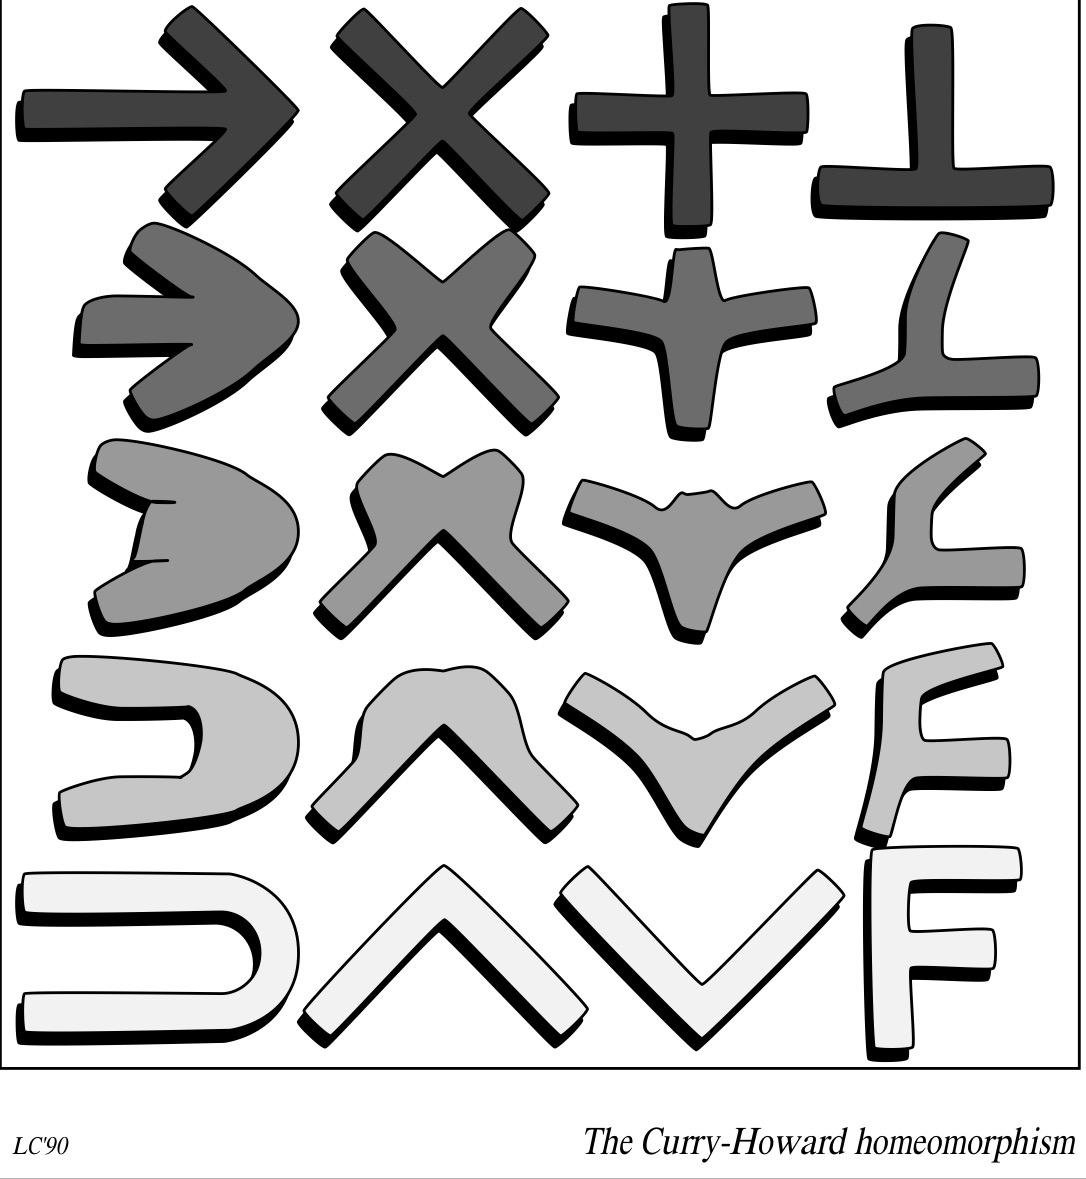
\includegraphics[scale=0.1]{defense-slides/cardelli-hc-corr.jpg}

      {{\tiny Source: \url{http://lucacardelli.name/Artifacts/Drawings/CurryHoward/CurryHoward.pdf}}}
    \end{figure}
\end{center}
\end{frame}

\begin{frame}[c]
  \frametitle{Bootstrapping: S O Intuitionistic Propositional Logic}
  \begin{center}
    \uncover<2->{{\LARGE \color{red}Propositions are truth values not resources}}\\
    \uncover<1->{
        \fbox{Language}
        \begin{flalign*}
          \text{Propositions and Connectives}\quad A, B, C &::= x \mid A \supset B \mid \forall x. B \mid A \vee B \mid A \wedge B \\
          \text{Context}\quad \Gamma,\Delta &::= \epsilon \mid \Gamma, A
        \end{flalign*}
        \fbox{Implicit Structural Rules}

        \begin{tabular}[h]{c c c}
          $A, B \vdash A$ &  $A, B \vdash B$   & Weakening \\

          \multicolumn{2}{c}{$A \vdash A \wedge A$} & Contraction \\

          \multicolumn{2}{c}{$A, B \vdash B, A$} & Exchange
        \end{tabular}
      }
  \end{center}
\end{frame}

\begin{frame}[c]
  \frametitle{Bootstrapping: Substructural Logic}
  \begin{center}
{\small     \begin{tabular}[h]{c c c c}
      System                                                                                 &  Who             & Year         & Control\\ \hline\hline
      Revelance Logic\footnote[frame]{{\tiny \fullcite{orlov_relevence_1928}}}               & Orlev            & 1928         & [WKN]\\
      Lambek Logic\footnote[frame]{{\tiny \fullcite{lambek_mathematics_1958}}}               & Lambek           & 1958         & [EXCH]\\
      Affine Logic\footnote[frame]{{\tiny \fullcite{grishin_affine_1974}}}                         & Grishin          & 1974         & [CTR] \\
      Linear Logic\footnote[frame]{{\tiny \fullcite{girard_linear_1987}}}                    & Girard           & 1987         & [WKN] [CTR]\\
      \color{red}{Logic of Bunched Implications}\footnote[frame]{{\tiny \fullcite{ohearn_logic_1999}}}    & \color{red}{O'Hearn and Pym}  & \color{red}{1999} & \color{red}{[WKN] [CTR]}\\
      Separation Logic \footnote[frame]{{\tiny \fullcite{reynolds_separation_2002}}}         & Reynolds         & 2002         & [WKN] [CTR] \\
      \vdots                                                                       & \vdots              & \vdots          & \vdots
    \end{tabular}
}  \end{center}
\end{frame}

\begin{frame}
  \frametitle{Bootstrapping: Logic of \BI{}}
  \begin{center}
    Coffee Shop

    1 cup coffee costs \$2

    \uncover<1->{
      \begin{tabular}[c]{c c c c c}
        \raisebox{-0.4\height}{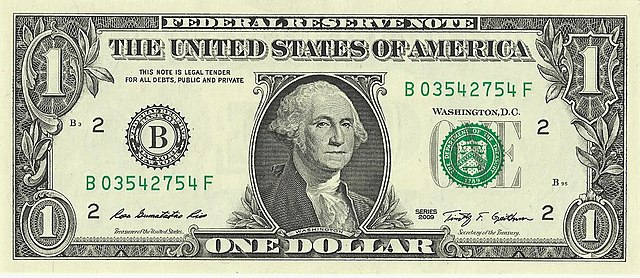
\includegraphics[scale=0.15]{defense-slides/one_usd}}
        & {\LARGE $,$}
        & \raisebox{-0.4\height}{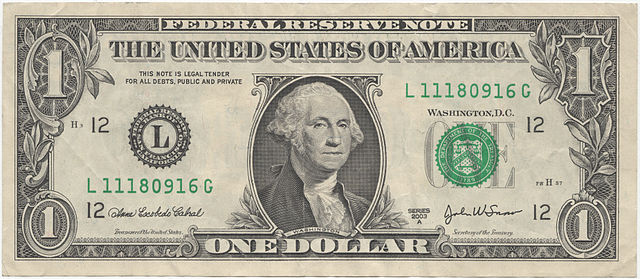
\includegraphics[scale=0.151]{defense-slides/one_usd_2}}
        & {\LARGE $\vdash$}
        & \raisebox{-0.4\height}{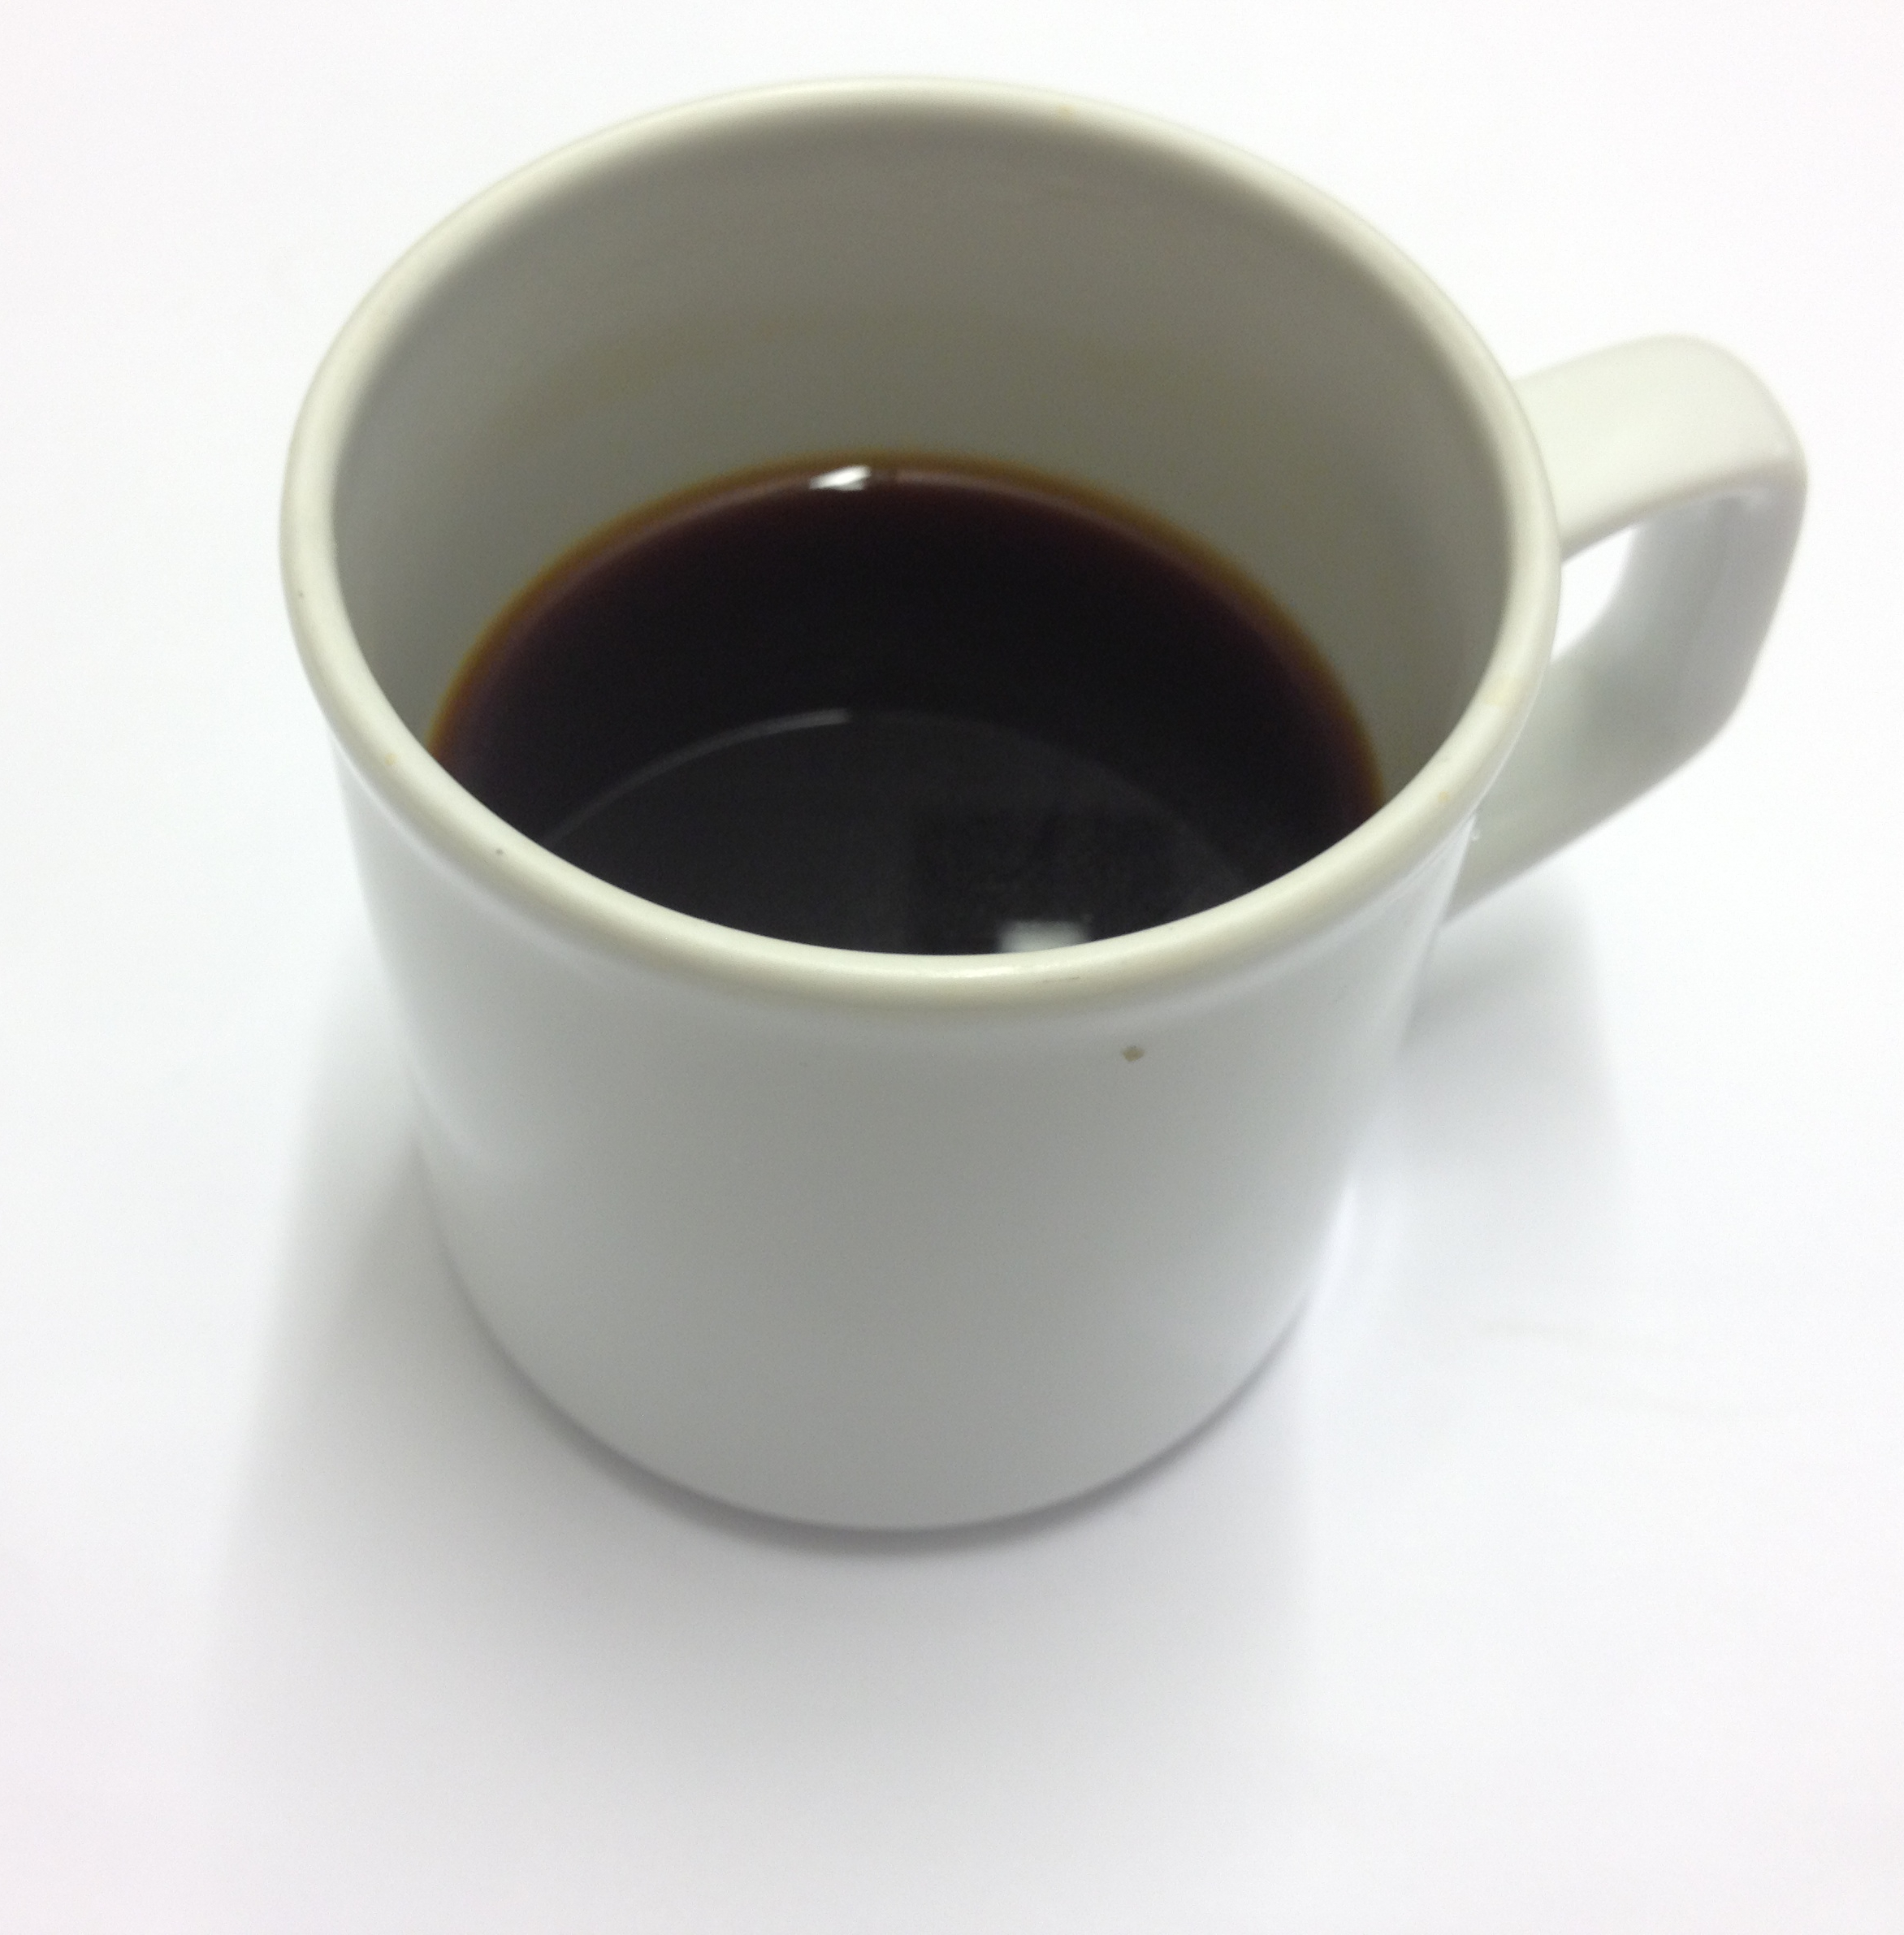
\includegraphics[scale=0.03]{defense-slides/coffee_cup}}
      \end{tabular}
    }
    \uncover<2->{
      \begin{tabular}[c]{c c c c c}
        \raisebox{-0.4\height}{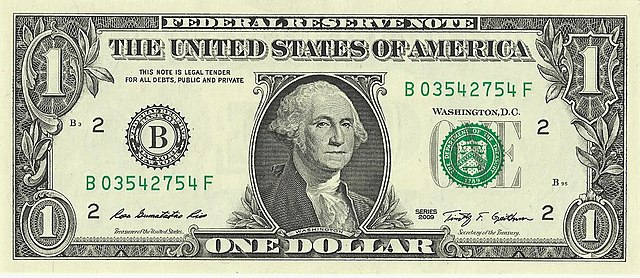
\includegraphics[scale=0.15]{defense-slides/one_usd}}
        & {\LARGE $,$}
        & \raisebox{-0.4\height}{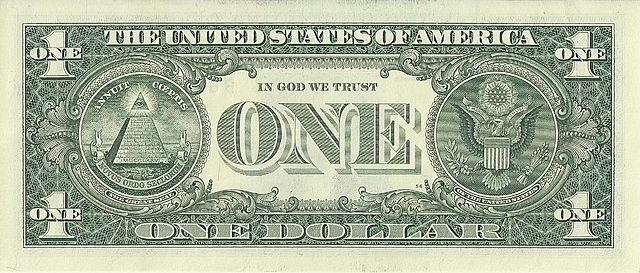
\includegraphics[scale=0.2]{defense-slides/one_usd_rev}}
        & {\LARGE $\not\vdash$}
        & \raisebox{-0.4\height}{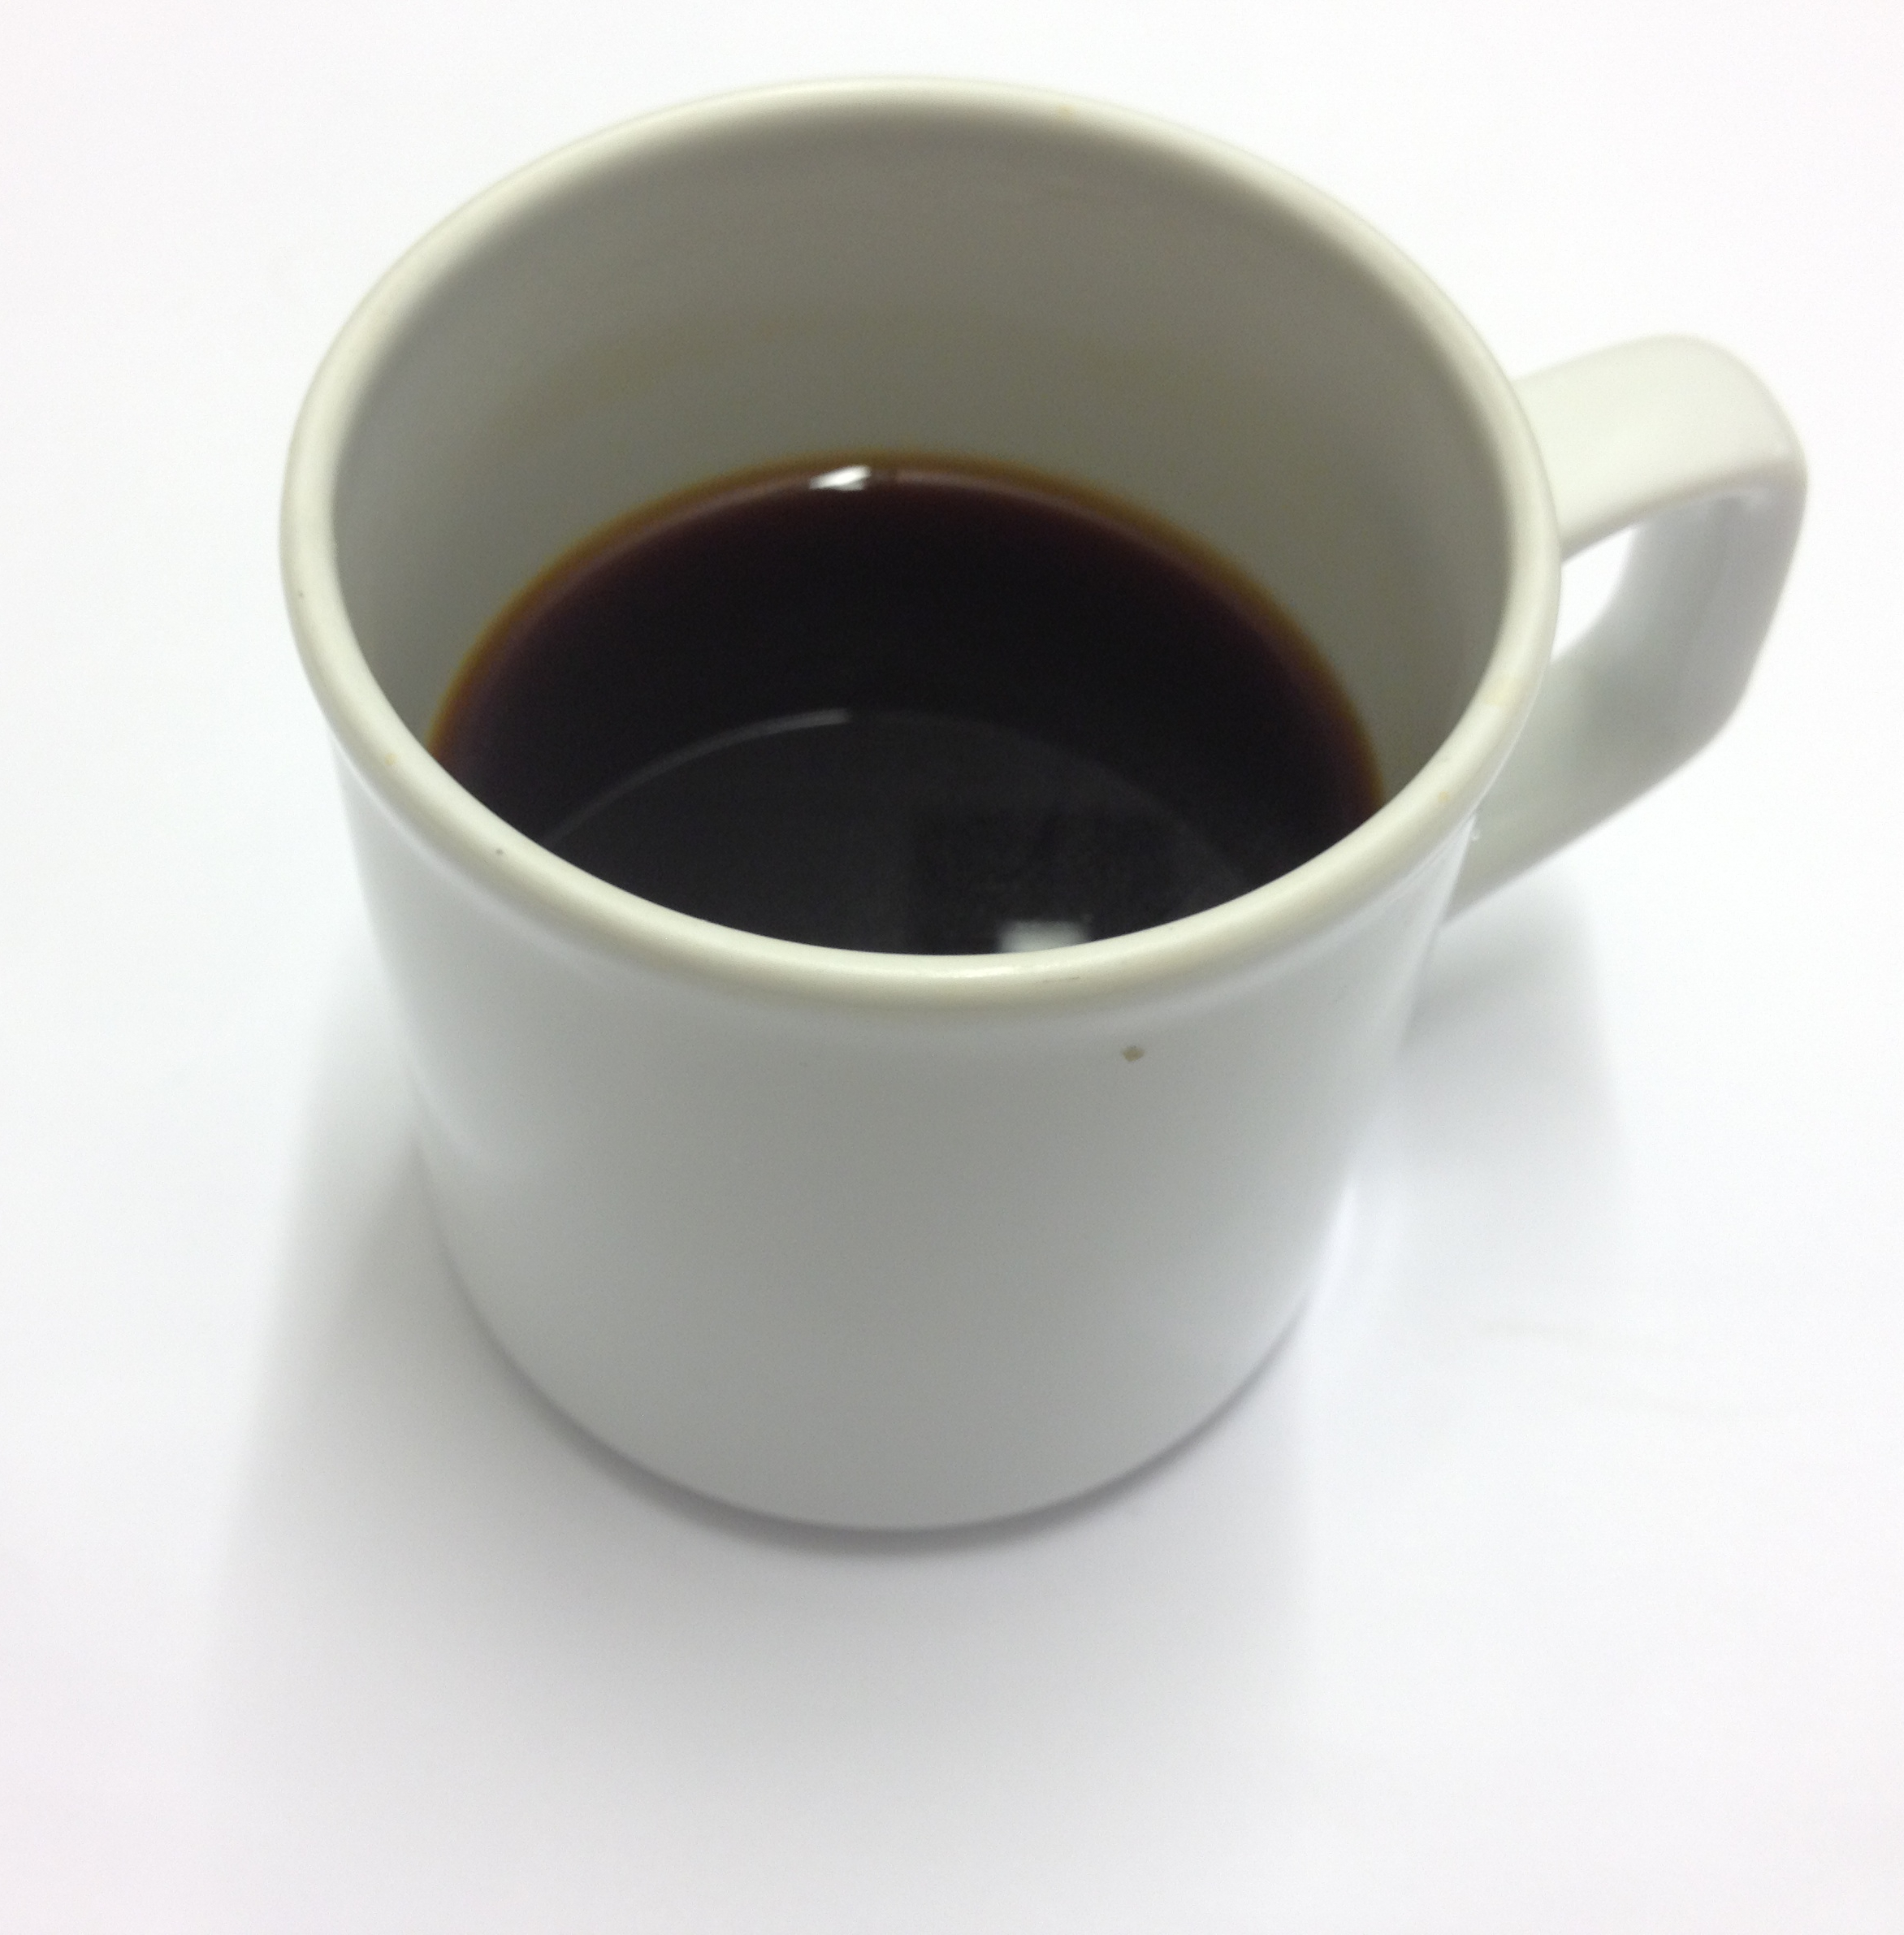
\includegraphics[scale=0.03]{defense-slides/coffee_cup}}
      \end{tabular}

      {\color{red}two separate} dollar bills necessary
    }
  \end{center}
\end{frame}

\begin{frame}[c]
  \frametitle{Bootstrapping: Logic of \BI{}}
  \begin{center}
    \begin{itemize}

    \item<1-> Conjunction ($\wedge$) split into two flavors
      \begin{center}
      \begin{tabular}[c]{c l}
      $A \otimes B$& A is separate from B\\
      $A \with B$&  A is a different view of B or A shares with B
      \end{tabular}
    \end{center}
    \item<2-> \BI{} contexts sensitive to different conjunction
      \begin{center}
        \begin{minipage}[h]{0.5\linewidth}
          $A, B \vdash A \otimes B$
        \end{minipage}%
        \begin{minipage}[h]{0.5\linewidth}
          $A; B \vdash A \with B$
        \end{minipage}
    \end{center}
    \item<3-> Contexts form trees, called bunches
      \begin{center}
        \begin{figure}[h]\centering
      \begin{minipage}{0.5\linewidth}\centering
        \tikzset{every tree node/.style={minimum width=2em},
          blank/.style={draw=none},
          edge from parent/.style=
          {draw,edge from parent path={(\tikzparentnode) -- (\tikzchildnode)}},
          level distance=1.5cm}
        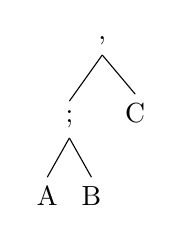
\begin{tikzpicture}
          \Tree
          [.,
          [.;
          [.A ]
          [.B ]
          ]
          [.C ]
          ]
        \end{tikzpicture}
        \caption*{$(A;B),C$}
      \end{minipage}%
      \begin{minipage}{0.5\linewidth}\centering
        \tikzset{every tree node/.style={minimum width=2em},
          blank/.style={draw=none},
          edge from parent/.style=
          {draw,edge from parent path={(\tikzparentnode) -- (\tikzchildnode)}},
          level distance=1.5cm}
        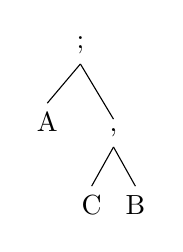
\begin{tikzpicture}
          \Tree
          [.;
          [.A ]
          [.,
          [.C ]
          [.B ]
          ]
          ]
        \end{tikzpicture}
        \caption*{$A;(B,C)$}
      \end{minipage}
    \end{figure}

    \end{center}

\end{itemize}
\end{center}
\end{frame}

\begin{frame}[c]
  \frametitle{Bootstrapping: Logic of \BI{}}
  \begin{center}
  Context connectives guide structural rules

  \begin{itemize}
  \item Contraction
    \begin{center}
      $A \vdash A;A$\\
      $A \not\vdash A,A$
    \end{center}

  \item Weakening
    \begin{center}
      $A;A \vdash A$ \qquad $A;B \vdash B$ \qquad $A;B \vdash A$\\
      $A,B \not\vdash A$ \qquad $A,B \not\vdash B$
    \end{center}
  \end{itemize}
\end{center}
\end{frame}

\begin{frame}
  \frametitle{Bootstrapping: Logic of \BI{}}
  \begin{center}
    Coffee Shop (Revisited)

    1 cup coffee costs \$2 \qquad  1 cookie costs \$1
    \begin{tabular}[c]{c c c c c}
        \raisebox{-0.4\height}{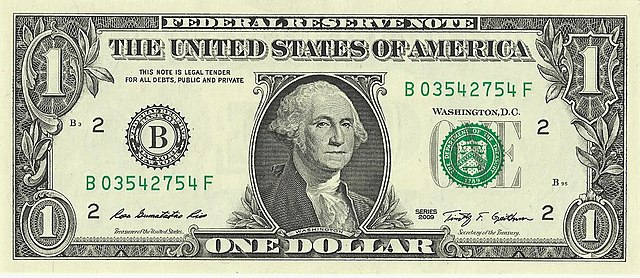
\includegraphics[scale=0.12]{defense-slides/one_usd}}
        & {\LARGE $\vdash$}
        & \raisebox{-0.4\height}{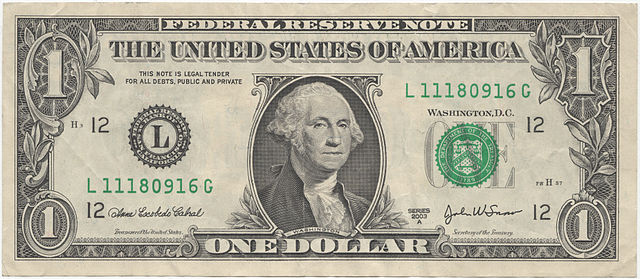
\includegraphics[scale=0.121]{defense-slides/one_usd_2}}
        & {\LARGE $\sepimp$}
        & \raisebox{-0.4\height}{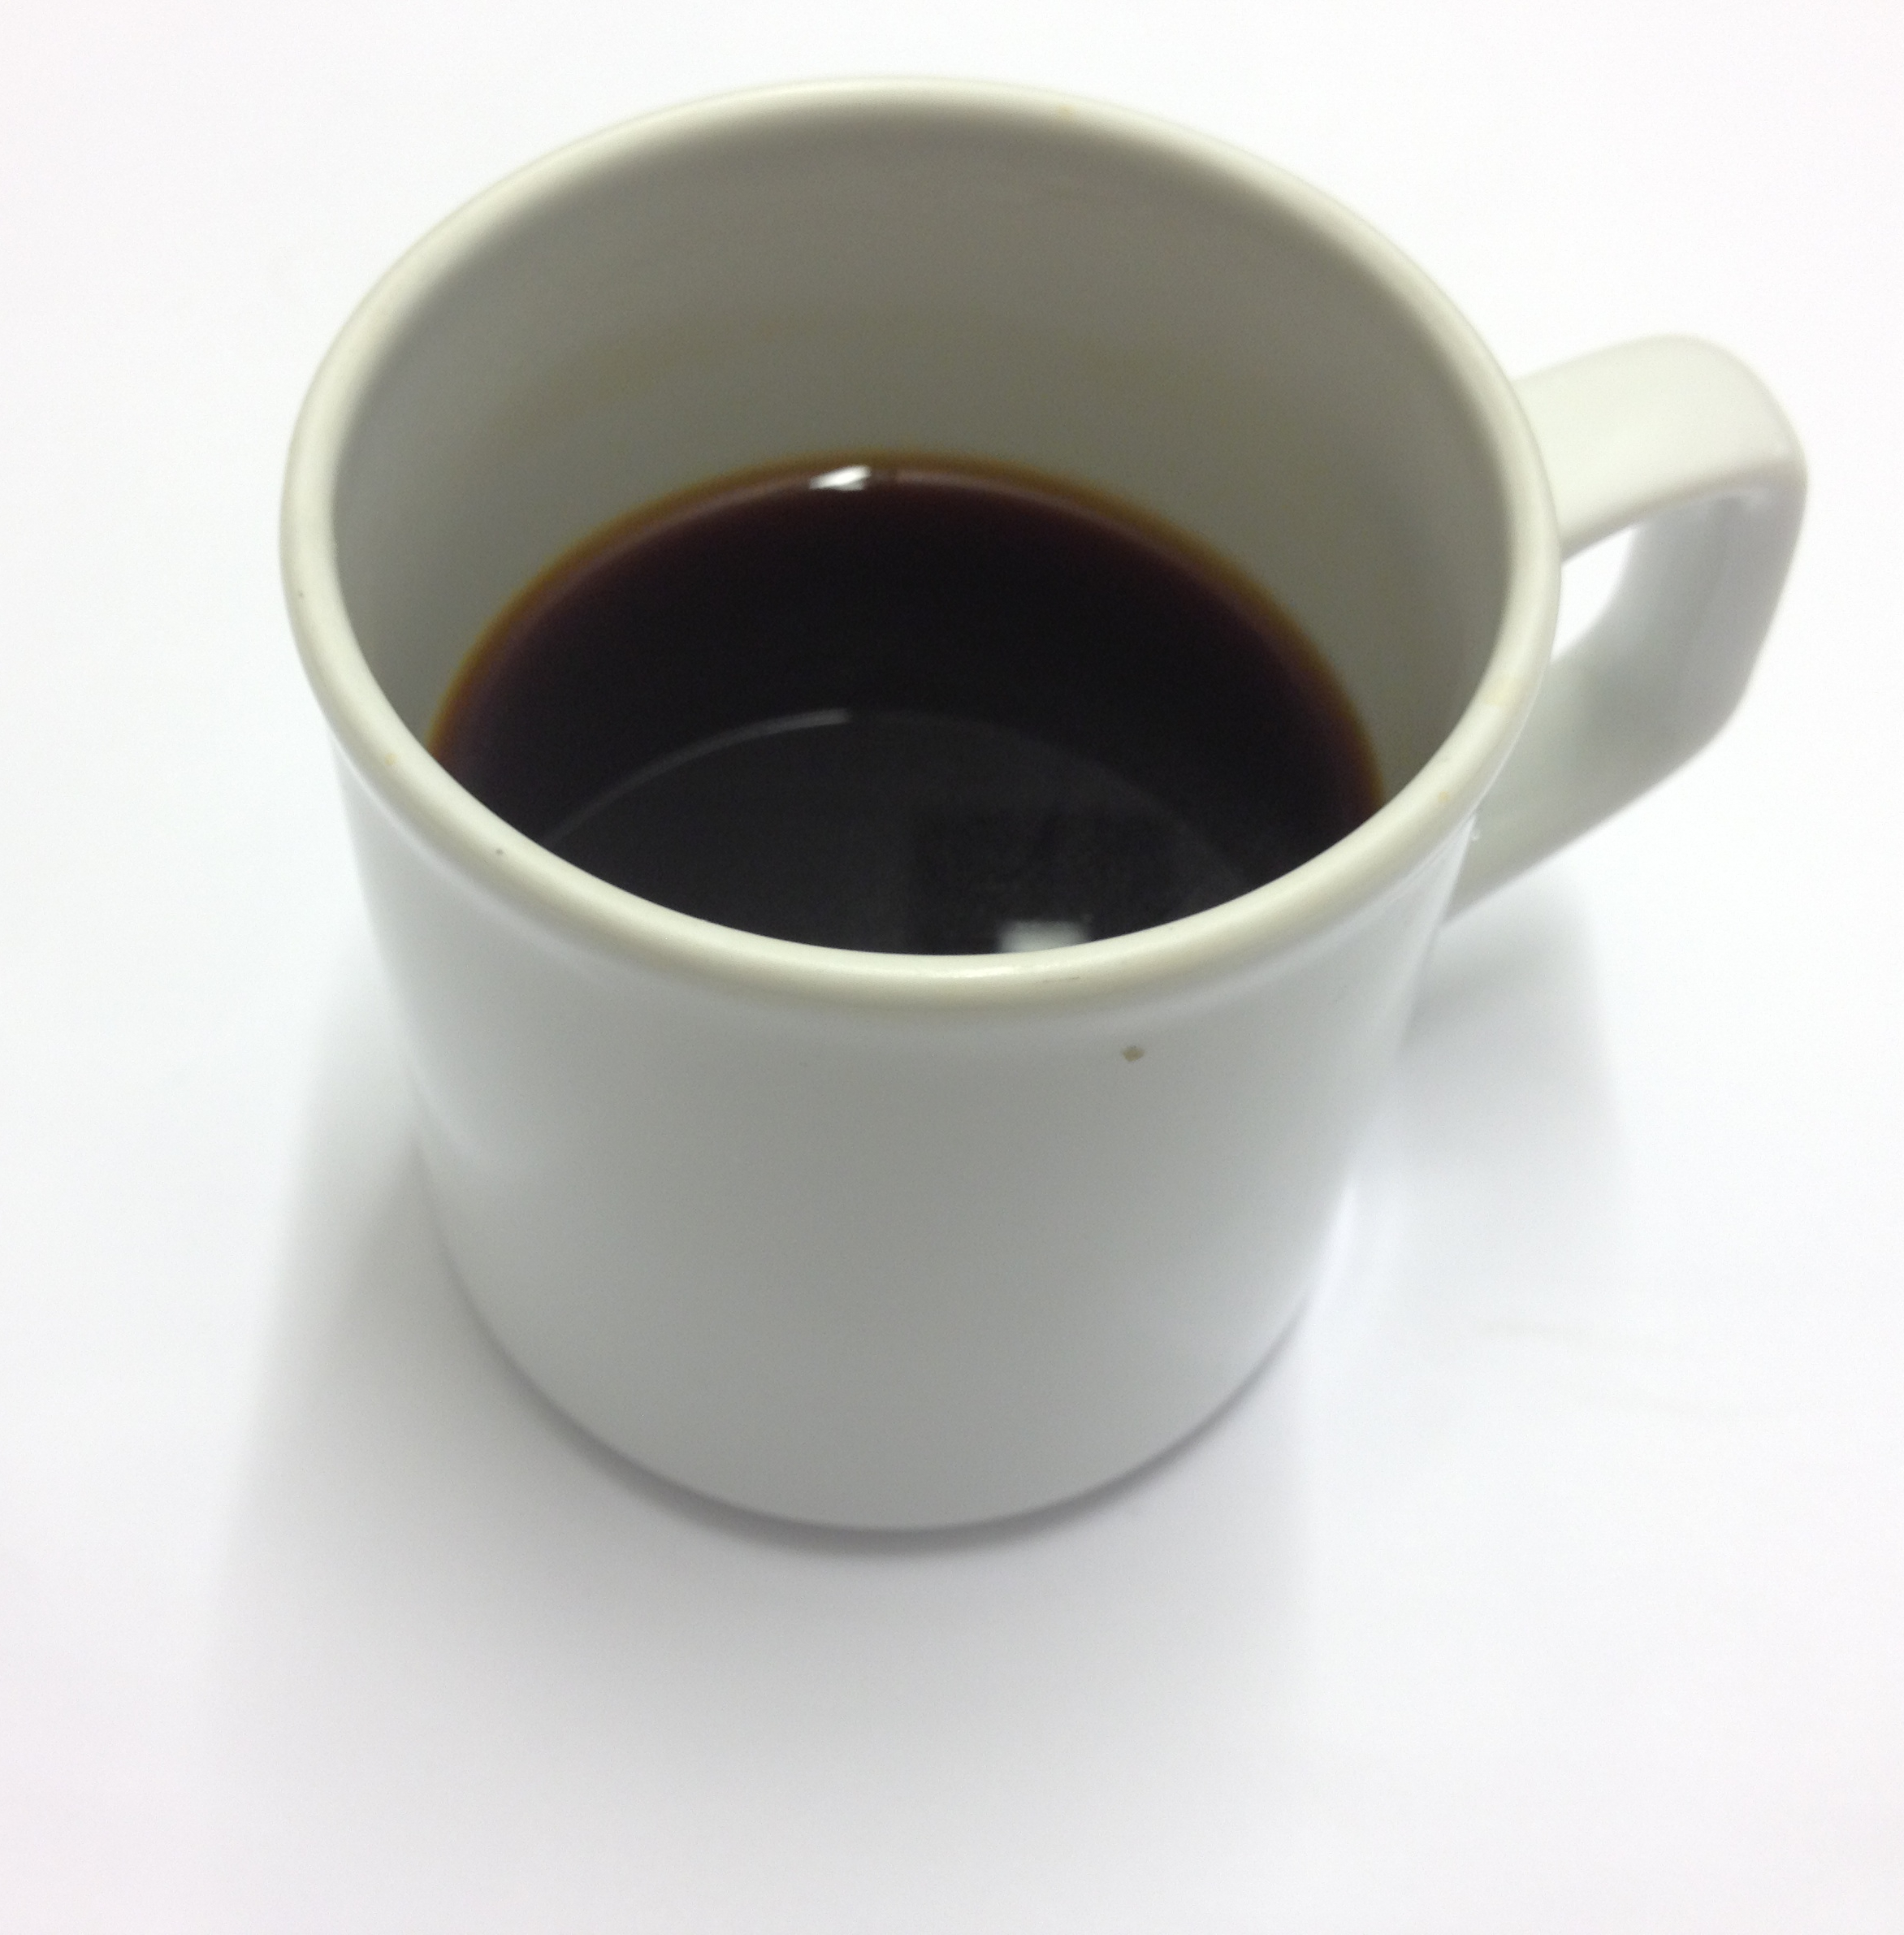
\includegraphics[scale=0.025]{defense-slides/coffee_cup}}
      \end{tabular}

      \begin{tabular}[c]{c c c c c}
        \raisebox{-0.4\height}{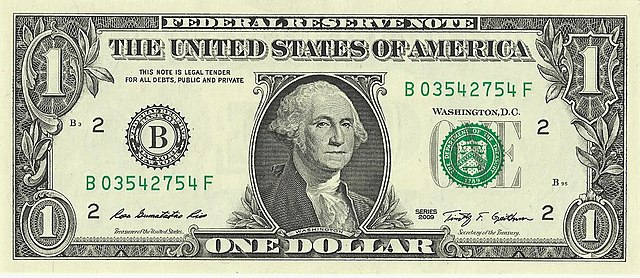
\includegraphics[scale=0.12]{defense-slides/one_usd}}
        & {\LARGE $\vdash$}
        & \raisebox{-0.4\height}{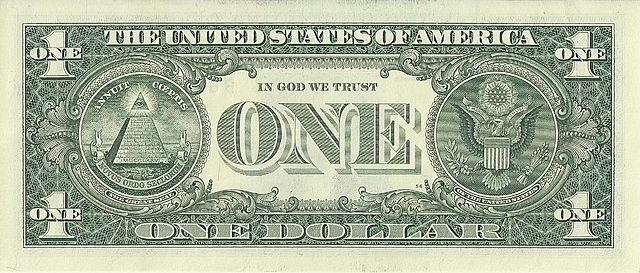
\includegraphics[scale=0.16]{defense-slides/one_usd_rev}}
        & {\LARGE $\shimp$}
        & \raisebox{-0.4\height}{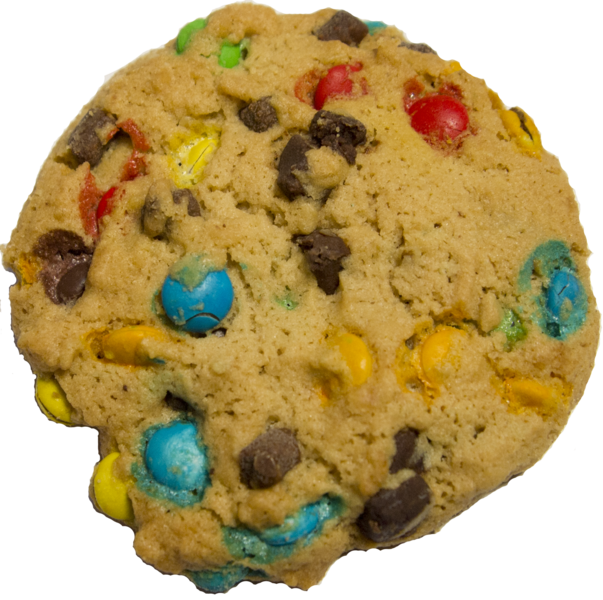
\includegraphics[scale=0.25]{defense-slides/cookie}}
      \end{tabular}

      \begin{tabular}[c]{c c c c c}
        \raisebox{-0.4\height}{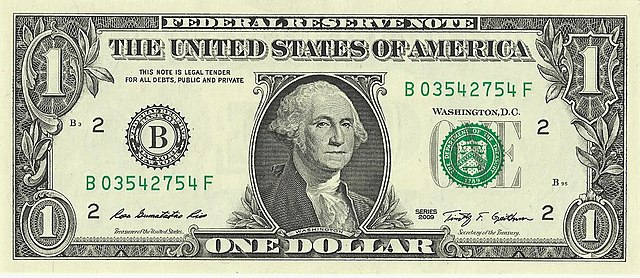
\includegraphics[scale=0.12]{defense-slides/one_usd}}
        & {\LARGE $\not\vdash$}
        & \raisebox{-0.4\height}{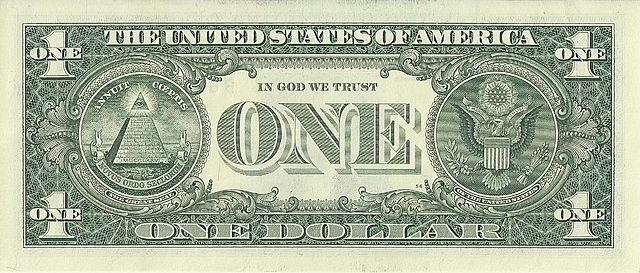
\includegraphics[scale=0.17]{defense-slides/one_usd_rev}}
        & {\LARGE $\shimp$}
        & \raisebox{-0.4\height}{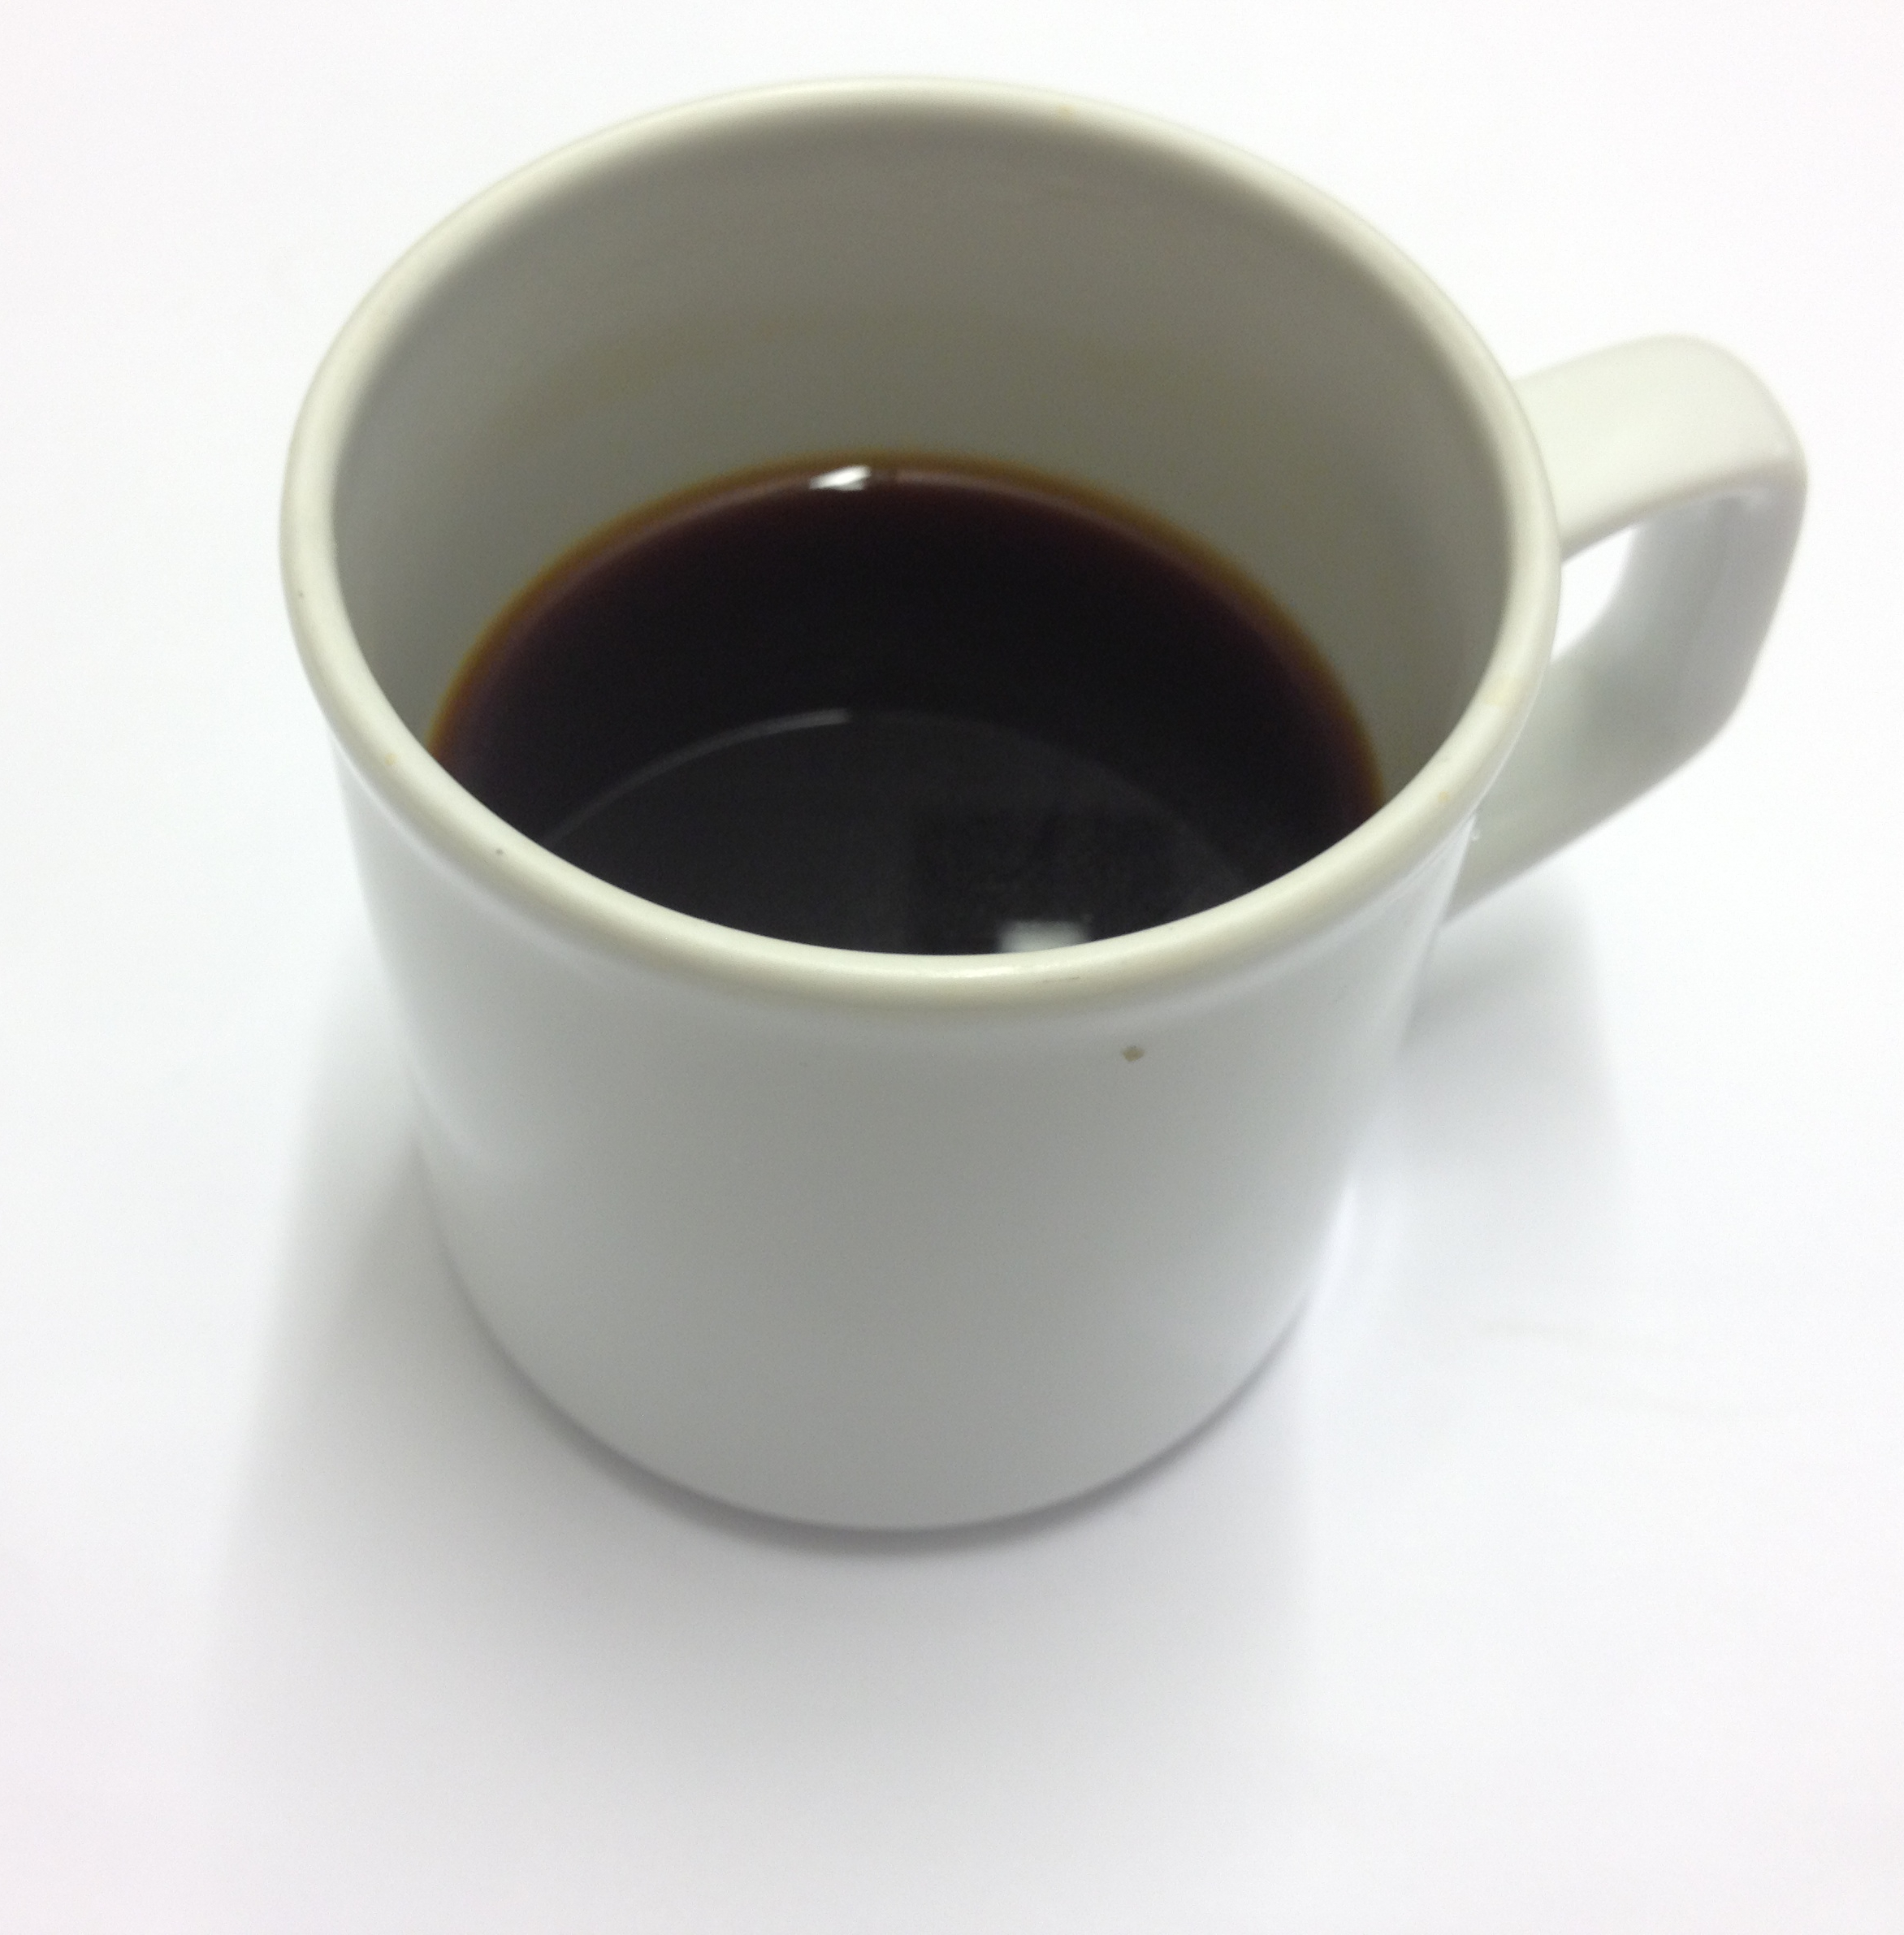
\includegraphics[scale=0.025]{defense-slides/coffee_cup}}
      \end{tabular}

  \end{center}
\end{frame}

\begin{frame}[c]
  \frametitle{Bootstrapping: Logic of \BI{}}
  \begin{center}
    Implications get corresponding flavors

    $A \otimes B \vdash C\ \text{iff}\ A \vdash B \sepimp C$

    $A \with B \vdash C\ \text{iff}\ A \vdash B \shimp C$
  \end{center}
\end{frame}


%%% Local Variables:
%%% mode: latex
%%% TeX-master: "defense-slides"
%%% End:


% Qub
% 10 mins
\section{\qub{}}\label{sec:qub}
% (10 min)

\begin{frame}[c]
  \frametitle{\qub{}}
  \begin{center}
{\LARGE      \qub{}: Curry-Howard interpretation of logic of \BI{}}
  \end{center}
\end{frame}

% \begin{frame}
%   \frametitle{\qub{}: Types and Predicates}
%   \begin{center}
%       \begin{minipage}{0.65\linewidth}
%     \begin{flalign*}
%       \text{Types}\ \ \  \tau, \upsilon, \phi         &::= t \mid \iota \mid \tau \rightarrow \tau\\
%       &\text{where}\qquad \rightarrow \in \{\tightoverset{\scalebox{0.5}{!}}{\sepimp}, \sepimp, \tightoverset{\scalebox{0.5}{!}}{\shimp}, \shimp \}\\
%       \text{Predicates}\ \ \        \pi,\omega        &::= \Un{\tau} \mid \ShFun{\phi} \mid \SeFun{\phi} \mid \tau \geq \tau' %\\
%       % { \color{battleshipgrey}
%       % \text{Qualified Types}\ \ \     \rho            &::= \tau \mid \pi => \rho \\
%       % \text{Type schemes}\ \ \        \sigma          &::= \rho \mid \forall t. \sigma
%       % }
%     \end{flalign*}
%   \end{minipage}

%   \begin{itemize}
%   \item $\SeFun{\phi}$: $\phi$ is a function that is separate from its argument
%   \item $\ShFun{\phi}$: $\phi$ is a function that is in sharing with its argument
%   \item $\Un{\tau}$: $\tau$ does not have resources or they can be copied/dropped easily
%   \end{itemize}
%   \end{center}
% \end{frame}


\begin{frame}
  \frametitle{\qub{}: Types}
  \begin{center}
    \begin{minipage}{0.65\linewidth}
      \begin{flalign*}
        \text{Types}\ \ \  \tau, \upsilon, \phi         &::= t \mid \iota \mid \tau \rightarrow \tau\\
        &\text{where}\qquad \rightarrow \in \{ \sepimp, \shimp \}\\
        % \text{Predicates}\ \ \        \pi,\omega        &::= \Un{\tau} \mid \ShFun{\phi} \mid \SeFun{\phi} \mid \tau \geq \tau' %\\
        % { \color{battleshipgrey}
        % \text{Qualified Types}\ \ \     \rho            &::= \tau \mid \pi => \rho \\
        % \text{Type schemes}\ \ \        \sigma          &::= \rho \mid \forall t. \sigma
        % }
    \end{flalign*}
    \end{minipage}
  \begin{itemize}
  \item $\sepimp$: Function type that is separate from its argument
  \item $\shimp$: Function type that is in sharing with its argument
  % \item $\tightoverset{\scalebox{0.5}{!}}{\sepimp}$, $\tightoverset{\scalebox{0.5}{!}}{\shimp}$: unrestricted versions of $\sepimp$ and $\shimp$
  \end{itemize}
  \end{center}
\end{frame}

\begin{frame}
  \frametitle{\qub{}: Expression Language}
  \begin{center}
    \begin{flalign*}
      \text{Term Variables}\ \ \  x, y, z  &\in \text{Variables} \nonumber\\
      \text{Expressions}\ \ \     M, N     &::= x \\
                                           & \mid \lambda^{\sepimp}x. M \mid \lambda^{\shimp}x. M \\
                                           & \mid M N
    \end{flalign*}
    \begin{itemize}
    \item $\lambda^{\sepimp}x. M$: Argument $x$ separate from $M$
    \item $\lambda^{\shimp}x. N$: Argument $x$ sharing with $M$
    \end{itemize}
  \end{center}
\end{frame}

\begin{frame}
  \frametitle{\qub{}: Typing Environment}
  \begin{center}
    \begin{itemize}
    \item Logic of \BI{}: Contexts are bunches
    \item \qub{}: Contexts generalized to graphs
    \end{itemize}
    {\small
      \begin{minipage}[c]{0.45\linewidth}
      \centering
      \tikzset{every tree node/.style={minimum width=2em},
        blank/.style={draw=none},
        edge from parent/.style=
        {draw,edge from parent path={(\tikzparentnode) -- (\tikzchildnode)}},
        level distance=1.5cm}
      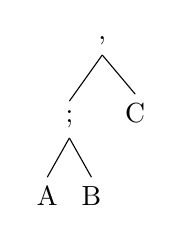
\begin{tikzpicture}
        \Tree
        [.,
        [.;
        [.A ]
        [.B ]
        ]
        [.C ]
        ]
      \end{tikzpicture}
    \end{minipage}\hfill%
    \begin{minipage}[c]{0.45\linewidth}
      \centering
      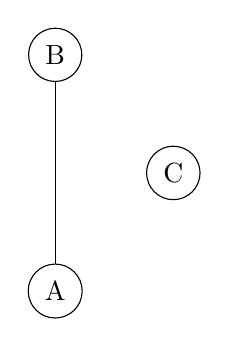
\begin{tikzpicture}
        \node[shape=circle,draw=black] (A) at (0,0) {A};
        \node[shape=circle,draw=black] (B) at (0,3) {B};
        \node[shape=circle,draw=black] (C) at (1.5,1.5) {C};

        \path [-] (A) edge node {} (B);
      \end{tikzpicture}
    \end{minipage}
  }
  \begin{itemize}
  \item Nodes are program objects
  \item (No) Edges represent (no) sharing
\end{itemize}
\end{center}
\end{frame}

\begin{frame}[fragile, c]
  \frametitle{\qub{}: Typing Environment}
  \begin{center}
    Sharing relation $\Psi$

    \begin{table}[h]
      \centering
      \begin{tabular}[c]{c c c}
      reflexive
      & $\forall x.\ x \mathbin{\Psi} x$
      & \raisebox{-0.4\height}{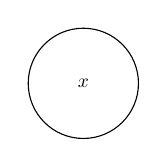
\begin{tikzpicture}[scale=0.7, fill=white, transform shape]
          \draw (0,0) circle  (1cm) node {$x$};
        \end{tikzpicture}}\\
      symmetric
      & $ \forall x, y.\ x \mathbin{\Psi} y \Rightarrow y \mathbin{\Psi} x$
      & \raisebox{-0.4\height}{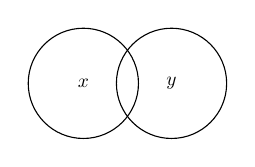
\begin{tikzpicture}[scale=0.7, fill=white, transform shape]
          \draw (0,0) circle  (1cm) node {$x$};
          \draw (1.6,0) circle  (1cm) node {$y$};
        \end{tikzpicture}}\\
      non-transitive
      & $\forall x, y, z.\ x \mathbin{\Psi} y \wedge y \mathbin{\Psi} z \not\Rightarrow x \mathbin{\Psi} z$
      & \raisebox{-0.4\height}{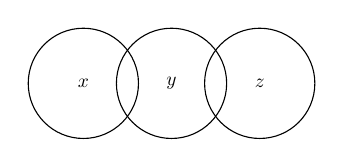
\begin{tikzpicture}[scale=0.7, fill=white, transform shape]
          \draw (0,0) circle  (1cm) node {$x$};
          \draw (1.6,0) circle  (1cm) node {$y$};
          \draw (3.2,0) circle  (1cm) node {$z$};
        \end{tikzpicture}}
      \end{tabular}
    \end{table}
\end{center}
\end{frame}

\begin{frame}[fragile, c]
  \frametitle{\qub{}: Typing Environment}
    \begin{itemize}
    \item \BI{} bunches need explicit transformations
      \begin{center}
      $ A; (B, C) \equiv (A;B),(A;C) $
      \end{center}
      \begin{center}
    {\small
      \begin{minipage}[c]{0.35\linewidth}
      \centering
      \tikzset{every tree node/.style={minimum width=2em},
        blank/.style={draw=none},
        edge from parent/.style=
        {draw,edge from parent path={(\tikzparentnode) -- (\tikzchildnode)}},
        level distance=1.5cm}
      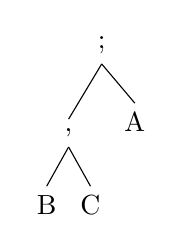
\begin{tikzpicture}
        \Tree
        [.;
        [.,
        [.B ]
        [.C ]
        ]
        [.A ]
        ]
      \end{tikzpicture}
    \end{minipage}%
    \begin{minipage}[c]{0.2\linewidth}
      \begin{center}
      {\LARGE $\rightsquigarrow$}\\
      {\LARGE $\rightsquigarrow$}\\
      {\LARGE $\rightsquigarrow$}
    \end{center}
    \end{minipage}%
    \begin{minipage}[c]{0.45\linewidth}
      \centering
 \tikzset{every tree node/.style={minimum width=2em},
        blank/.style={draw=none},
        edge from parent/.style=
        {draw,edge from parent path={(\tikzparentnode) -- (\tikzchildnode)}},
        level distance=1.5cm}
      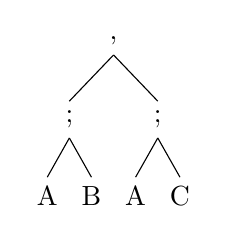
\begin{tikzpicture}
        \Tree
        [.,
        [.;
        [.A ]
        [.B ]
        ]
        [.;
        [.A ]
        [.C ]
        ]
        ]
      \end{tikzpicture}
    \end{minipage}
  }
\end{center}


\item \qub{} sharing graphs internalize the transformation
  \begin{center}
      {\small
    \begin{minipage}[c]{1\linewidth}
      \centering
      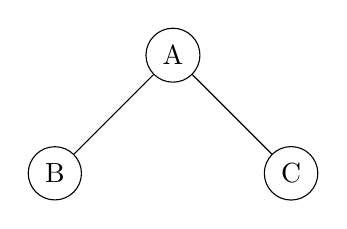
\begin{tikzpicture}
        \node[shape=circle,draw=black] (A) at (1.5,3) {A};
        \node[shape=circle,draw=black] (B) at (0,1.5) {B};
        \node[shape=circle,draw=black] (C) at (3,1.5) {C};

        \path [-] (A) edge node {} (B);
        \path [-] (A) edge node {} (C);
      \end{tikzpicture}
    \end{minipage}
  }
\end{center}

\end{itemize}
\end{frame}


\begin{frame}
  \frametitle{\qub{}: Typing Environment}
  \begin{center}
    Adjacency lists for sharing graphs

    ``$x$ of type $\sigma$ is in sharing with $\vec{y}$''

    $(x, \sigma, \vec{y}) \in \Gamma$
    \begin{flalign*}
      \text{Typing Context}\ \ \      \Gamma,\Delta     &::= \epsilon \mid \Gamma, x^{\vec{y}}:\sigma
    \end{flalign*}

  \end{center}
\end{frame}


%%% Local Variables:
%%% mode: latex
%%% TeX-master: "defense-slides"
%%% End:


% Examples. Did we solve our problem?
% 5 mins
\section{Examples And Extensions}\label{sec:examples}

\begin{frame}
  \frametitle{Examples: $\lambda$-encoding standard structures}
  \begin{itemize}
  \item Multiplicative Product (Separating Pair)
      \begin{flalign*}
      \tau \otimes \tau' &= \tau \sepimp \tau' \sepimp (\tau \sepimp \tau' \sepimp \upsilon) \sepimp \upsilon\\
      \Pair{x,y} &= \lambda^{\sepimp}  x. \lambda^{\sepimp}  y. \lambda^{\sepimp}  f. f x y
    \end{flalign*}
  \item Additive Product  (Sharing Pair)
    \begin{flalign*}
      \tau \with \tau' &= \tau \sepimp \tau' \shimp (\tau \sepimp \tau' \shimp \upsilon) \shimp \upsilon\\
      \Pair{x;y} &= \lambda^{\sepimp}  x. \lambda^{\shimp} y. \lambda^{\shimp} f. f x y
    \end{flalign*}
  \item Sums
    \begin{flalign*}
      \tau \oplus \tau' &= (\tau \sepimp \upsilon) \rightarrow (\tau' \shimp \upsilon) \shimp \upsilon\\
      \texttt{case}\ {c}\ \texttt{of}\ {\{ f;g \}} &= \lambda^{\sepimp}c. \lambda^{\shimp}f. \lambda^{\shimp}g. c f g
    \end{flalign*}
    \begin{minipage}[h]{0.45\linewidth}
      \begin{flalign*}
        \Inl{} &: \tau \sepimp (\tau \oplus \tau')\\
        \Inl{} &= \lambda^{\sepimp} x. \lambda^{\shimp} f. \lambda^{\shimp} g. f x
      \end{flalign*}
    \end{minipage}%
    \begin{minipage}[h]{0.45\linewidth}
      \begin{flalign*}
        \Inr{} &: \tau' \sepimp (\tau \oplus \tau')\\
        \Inr{} &= \lambda^{\sepimp} y. \lambda^{\shimp} f. \lambda^{\shimp} g. g y
      \end{flalign*}
    \end{minipage}
  \end{itemize}
\end{frame}

\begin{frame}[c, fragile]
  \frametitle{\qub{}: Extension}
  \begin{center}
   {\large Towards programmer friendly}
   \begin{itemize}
   \item<1-> Define custom types

   \begin{haskell}
                  data Bool   = True | False
                  data List a = Nil  | Cons a a
                  data Tree a = Leaf | Node a a
                               $\vdots$
   \end{haskell}
   \item<2-> Type classes, functional dependencies
    \begin{haskell}
                 class Monad m a  where
                      return      :: a -> m a
                      ($\gg\!=$)  :: a -> (a -> m b) -> m b

                 class Collection e co | co -> e where
                      empty :: co
                      insert :: e -> co -> co
                      member :: e -> co -> Bool
                              $\vdots$
   \end{haskell}
 \end{itemize}

 \end{center}
\end{frame}


\begin{frame}[c]
  \frametitle{More Bootstrapping: Qualified Types and Kinds}
  \begin{itemize}
  \item Incorporate predicates into type language for finer grained
    polymorphism
    % {\large   $\Gamma \vdash M:\sigma $}
    % ``Type of $M$ is $\sigma$\\
    % and $\Gamma$ specifies the free variables in $M$\footnote[frame]{\fullcite{jones_theory_1994}}''
    \begin{center}
      $P \mid \Gamma \vdash M:\sigma$
    \end{center}
    % ``Type of $M$ is $\sigma$\\
    % when predicates in $P$ are satisfied\\
    % and $\Gamma$ specifies the free variables in $M$\footnote[frame]{\fullcite{jones_theory_1994}}''
  \item Incorporate kinds, build hierarchy over types and generalize types to type constructors\footnote[frame]{\fullcite{barendregt_1991, jones_system_1993}}
    \begin{center}
      \begin{flalign*}
        \text{Kinds}\ \ \                    \kappa       &::= \star \mid \kappa' \rightarrow \kappa\\
        \text{Types}\ \ \ \tau^{\kappa}, \phi^{\kappa}      &::= t^\kappa \mid T^{\kappa} \mid \tau^{\kappa' \rightarrow \kappa}\tau^{\kappa'}\\
        \text{Type Constructors}\ \ \   T^{\kappa}         &\in \mathcal{T}^{\kappa}\quad \text{where}\quad T^{\kappa} \subseteq \dots
      \end{flalign*}
    \end{center}
  \end{itemize}
\end{frame}

% \begin{frame}[c]
%   \frametitle{More Bootstrapping: Qualified Types}
%   \begin{center}
%   {\LARGE   $${\color{red}P} \mid \Gamma \vdash M:\sigma $$}
% ``Type of $M$ is $\sigma$\\
%   when predicates in $P$ are satisfied\\
%   and $\Gamma$ specifies the free variables in $M$''\footcite{jones_theory_1994}

%   Incorporate predicates into type language for finer grained polymorphism


%   {\LARGE $(P \mid \sigma)$}

%   Instances of $\sigma$ that satisfy P
%   \end{center}
% \end{frame}

% \begin{frame}
%   \frametitle{More Bootstrapping: Quill}
%   \begin{center}
%     Quill\footcite{morris_best_2016}: {\color{blue}Qu}al{\color{blue}i}fied types + {\color{blue}l}inear {\color{blue}l}ogic\\
%   \end{center}
%   Predicates:
%   \begin{itemize}
%   \item $\Un{\tau}$\quad If $\tau$ does not have resources
%     or can be copied or dropped easily.
%   \item $\Fun{\tau}$\quad If $\tau$ is a function type
%   \item $\tau \geq \tau'$\quad If $\tau$ less restricting than $\tau'$
%   \end{itemize}
% \end{frame}

% \begin{frame}[fragile, c]
%   \frametitle{More Bootstrapping: Quill}
%   \begin{center}
%     Quill\footcite{morris_best_2016}: {\color{blue}Qu}al{\color{blue}i}fied types + {\color{blue}l}inear {\color{blue}l}ogic\\
%   \end{center}
%   Qualifying Types:
%   \begin{itemize}
%   \item Unrestricted Types: $\Un{\texttt{Int}}$, $\Un{\text{Bool}}$
%   \item Restricted or Linear Types: FileHandle
%   \item Function Types: $\Fun{(\texttt{Int} \rightarrow \texttt{Int})}$,
%     $\Fun{(\texttt{String} \rightarrow \texttt{String})}$
%   \end{itemize}
% \end{frame}

\begin{frame}
  \frametitle{\qub{}: Types and Predicates}
  \begin{center}
      \begin{minipage}{0.65\linewidth}
    \begin{flalign*}
      \text{Types}\ \ \  \tau, \upsilon, \phi         &::= t \mid \iota \mid \tau \rightarrow \tau\\
      &\text{where}\qquad \rightarrow \in \{\tightoverset{\scalebox{0.5}{!}}{\sepimp}, \sepimp, \tightoverset{\scalebox{0.5}{!}}{\shimp}, \shimp \}\\
      \text{Predicates}\ \ \        \pi,\omega        &::= \Un{\tau} \mid \ShFun{\phi} \mid \SeFun{\phi}\\% \mid \tau \geq \tau' %\\
      % { \color{battleshipgrey}
      % \text{Qualified Types}\ \ \     \rho            &::= \tau \mid \pi => \rho \\
      % \text{Type schemes}\ \ \        \sigma          &::= \rho \mid \forall t. \sigma
      % }
    \end{flalign*}
  \end{minipage}

  \begin{itemize}
  \item $\SeFun{\phi}$: $\phi$ is a function that is separate from its argument
  \item $\ShFun{\phi}$: $\phi$ is a function that is in sharing with its argument
  \item $\Un{\tau}$: $\tau$ does not have resources or they can be copied/dropped easily\footnote[frame]{\fullcite{morris_best_2016}}
  \end{itemize}
  \end{center}
\end{frame}


\begin{frame}
  \frametitle{\qub{}: Types and Predicates}
  \begin{center}
    \begin{minipage}{0.65\linewidth}
      \begin{flalign*}
        \text{Types}\ \ \  \tau, \upsilon, \phi         &::= t \mid \iota \mid \tau \rightarrow \tau\\
        &\text{where}\qquad \rightarrow \in \{\tightoverset{\scalebox{0.5}{!}}{\sepimp}, \sepimp, \tightoverset{\scalebox{0.5}{!}}{\shimp}, \shimp \}\\
        \text{Predicates}\ \ \        \pi,\omega        &::= \Un{\tau} \mid \ShFun{\phi} \mid \SeFun{\phi}\\% \mid \tau \geq \tau' %\\
        % { \color{battleshipgrey}
        % \text{Qualified Types}\ \ \     \rho            &::= \tau \mid \pi => \rho \\
        % \text{Type schemes}\ \ \        \sigma          &::= \rho \mid \forall t. \sigma
        % }
    \end{flalign*}
    \end{minipage}
  \begin{itemize}
  \item $\sepimp$: Function type that is separate from its argument
  \item $\shimp$: Function type that is in sharing with its argument
  \item $\tightoverset{\scalebox{0.5}{!}}{\sepimp}$, $\tightoverset{\scalebox{0.5}{!}}{\shimp}$: Unrestricted versions of $\sepimp$ and $\shimp$
  \end{itemize}
  \end{center}
\end{frame}


% \begin{frame}
%   \frametitle{\qub{}: Extension}
%   \begin{itemize}
%   \item Kind System with type constructors and qualified types\cite{barendregt_1991, mark_type_2000}
%     \begin{flalign*}
%                                            t, u         &\in \text{Type Variables}\\
%       \text{Kinds}\ \ \                    \kappa       &::= \star \mid \kappa' \rightarrow \kappa\\
%       \text{Types}\ \ \ \tau^{\kappa}, \phi^{\kappa}      &::= t^\kappa \mid T^{\kappa} \mid \tau^{\kappa' \rightarrow \kappa}\tau^{\kappa'}\\
%       \text{Type Constructors}\ \ \   T^{\kappa}       &\in \mathcal{T}^{\kappa} \\
%                   &\text{where}\quad\{\otimes, \with, \oplus, \tightoverset{\scalebox{0.5}{!}}{\sepimp}, \sepimp, \tightoverset{\scalebox{0.5}{!}}{\shimp}, \shimp \} \subseteq \mathcal{T}^{\star \rightarrow \star \rightarrow \star}\\
%       \text{Predicates}\ \ \          \pi, \omega     &::= \Un{\tau} \mid \SeFun{\phi} \mid \ShFun{\phi} \mid \tau \geq \tau' \\
%       % \text{Qualified Types}\ \ \     \rho            &::= \tau^{\star} \mid \pi => \rho \\
%       % \text{Type schemes}\ \ \        \sigma          &::= \rho \mid \forall t. \sigma
%     \end{flalign*}
%   \end{itemize}
% \end{frame}


\begin{frame}[fragile, c]
  \frametitle{\qub{}: Datatypes with Sharing and Separation}
  \begin{center}
    \fbox{Sharing Pair}\\

    \begin{tabular}[c]{c}
           \begin{haskell}
data ShPair a b = ShP a; b     {- ; for sharing -}

fst :: ShPair a b ->> a
fst (ShP a b) = a              {- Succeeds typecheck -}

snd :: ShPair a b ->> b
snd (ShP a b) = b              {- Succeeds typecheck -}

swap :: ShPair a b ->> ShPair b a
swap (ShP a b) = ShP b a       {- Succeeds typecheck -}
          \end{haskell}
        \end{tabular}
  \end{center}
\end{frame}

\begin{frame}[fragile, c]
  \frametitle{\qub{}: Datatypes with Sharing and Separation}
  \begin{center}
    \fbox{Separating Pair}
       \begin{tabular}[c]{c}
          \begin{haskell}
data SePair a b = SeP a, b     {- , for separation -}

@fst :: SePair a b ${\color{red}\sepimp}$ a
fst (SeP a b) = a              {- Fails typecheck -}@

@snd :: SePair a b ${\color{red}\sepimp}$ b
snd (SeP a b) = b              {- Fails typecheck -}@

swap :: SePair a b $\sepimp$ SePair b a
swap (SeP a b) = SeP b a       {- Succeeds typecheck -}
          \end{haskell}
        \end{tabular}
  \end{center}
\end{frame}

%%% Local Variables:
%%% mode: latex
%%% TeX-master: "defense-slides"
%%% End:


% Conclusion and future work
% 2 mins
\section{Conclusion and Future Work}\label{sec:conclusion}

\begin{frame}[fragile, c]
  \frametitle{Motivation Revisited}
  \begin{center}
    {\LARGE
      What about filehandles, exceptions and memory leaks and runtime crashes?
    }
\end{center}

\end{frame}

\begin{frame}[fragile, c]
  \frametitle{Filehandles Revisited}
  \begin{center}
  File Handling API in \qub{}
  \begin{haskell}
     openFile  :: FilePath   $\sepimp$ IO FileHandle

     closeFile :: FileHandle $\sepimp$ IO ()

     readLine  :: FileHandle $\sepimp$ IO (String, FileHandle)

     writeLine :: FileHandle $\sepimp$ String
                             $\sepimp$ IO FileHandle




     ($\gg\!=$) :: IO a $\sepimp$ (a $\sepimp$ IO b) $\sepimp$ IO b
   \end{haskell}
\end{center}
\end{frame}

\begin{frame}[fragile, c]
  \frametitle{Filehandles Revisited}
  \begin{center}
  {\LARGE \color{white}Fails Typecheck!}

  \begin{haskell}
               do f  <- openFile "sample.txt"
                  (s, f)  <- readLine f
                  () <- closeFile f
                  () <- closeFile f
            \end{haskell}
{\LARGE      $\downlsquigarrow \qquad \downlsquigarrow \qquad \downlsquigarrow$}
            \begin{haskell}
               ($\gg\!=$) (openFile "sample.txt") (\ f ->

               ($\gg\!=$) (readLine f) (\ (s, f) ->

               ($\gg\!=$) (closeFile f) (\ _ -> closeFile f)
            \end{haskell}
          \end{center}

\end{frame}

\begin{frame}[fragile, c]
  \begin{center}
  {\LARGE \color{white}Fails Typecheck!}

  \frametitle{Filehandles Revisited}
\begin{haskell}
               do f  <- openFile "sample.txt"
                  (s, f)  <- readLine f
                  () <- closeFile f
                  () <- closeFile f
               \end{haskell}
{\LARGE      $\downlsquigarrow \qquad \downlsquigarrow \qquad \downlsquigarrow$}
               \begin{haskell}
               ($\gg\!=$) (openFile "sample.txt") (\ f ->

               ($\gg\!=$) (readLine f) (\ (s, f) ->

               @(${\color{red}\gg\!=}$) (closeFile f) (\ _ -> closeFile f)@
               \end{haskell}
          \end{center}

\end{frame}

\begin{frame}[fragile, c]
  \begin{center}
  \frametitle{Filehandles Revisited}
  {\LARGE \color{red}Fails Typecheck!}

\begin{haskell}
                do f  <- openFile "sample.txt"
                   (s, f)  <- readLine f
                   () <- closeFile f
                   () <- closeFile f
               \end{haskell}
{\LARGE      $\downlsquigarrow \qquad \downlsquigarrow \qquad \downlsquigarrow$}
               \begin{haskell}
               {- (${\color{dkgreen}\gg\!=}$) :: IO a ${\color{dkgreen}\sepimp}$ (a ${\color{dkgreen}\sepimp}$ IO b) ${\color{dkgreen}\sepimp}$ IO b -}
               ($\gg\!=$) (openFile "sample.txt") (\ f ->
               {- (${\color{dkgreen}\gg\!=}$) :: IO a ${\color{dkgreen}\sepimp}$ (a ${\color{dkgreen}\sepimp}$ IO b) ${\color{dkgreen}\sepimp}$ IO b -}
               ($\gg\!=$) (readLine f) (\ (s, f) ->
               {- (${\color{dkgreen}\gg\!=}$) :: IO a ${\color{dkgreen}\sepimp}$ (a ${\color{dkgreen}\sepimp}$ IO b) ${\color{dkgreen}\shimp}$ IO b -}
               @(${\color{red}\gg\!=}$) (closeFile f) (\ _ -> closeFile f)@
\end{haskell}
\end{center}
\end{frame}

\begin{frame}[fragile, c]
  \frametitle{Exceptions Revisited}
  \begin{center}
    \begin{haskell}
          openFile :: FilePath $\sepimp$ IO FileHandle
          closeFile :: FileHandle $\sepimp$ IO ()
          readFile :: FileHandle $\sepimp$ IOF (String, FileHandle)
          writeFile :: String $\sepimp$ FileHandle $\sepimp$ IOF FileHandle

          throw :: Exception $\sepimp$ IOF a
          catch :: IOF a $\sepimp$ (Exception $\sepimp$ IO a) ->> IO a
          \end{haskell}
\begin{itemize}
\item May not fail \texttt{IO a}
\item May fail \texttt{IOF a}
\end{itemize}
\end{center}
\end{frame}

\begin{frame}[fragile, c]
  \frametitle{Exceptions Revisited}
  \begin{center}
    \begin{haskell}
          readFromFile :: FilePath $\sepimp$ IO (Either String String)
          readFromFile fpath =
          do @fh@  <- openFile fpath
             ((s, @fh@)  <- readLine @fh@
             let l = caps s
             () <- closeFile @fh@
             return \dollar Right l) `catch`
                     (\e -> do closeFile @fh@
                               return \dollar Left "Could not read file")
                        \end{haskell}
                      \end{center}
     \begin{itemize}
     \item Filehandle \texttt{fh} is shared between the \texttt{catch} arguments
       \begin{haskell}
         catch :: IOF a $\sepimp$ (Exception $\sepimp$ IO a) ->> IO a
       \end{haskell}
     \item Avoids memory leak
\end{itemize}
\end{frame}


\begin{frame}
  \frametitle{Contributions revisited}

  \begin{itemize}

  \item {\color{red}Language design}
    \begin{itemize}
    \item {\color{red}Resources are ``first class citizens''}
    \item {\color{red}Resources(variables) can be in sharing or separate}
    \end{itemize}

  \item {\color{red}\qub{} is logic of \BI on steroids}
    \begin{itemize}
    \item {\color{red}Typing Environments as graphs}
    \end{itemize}
  \item {\color{red}Working examples}
  \item Formalizing and proving important properties of \qub{}
    \begin{itemize}
    \item Type system
    \item Syntax directed type system (sound and complete)
    \item Type inference algorithm $\M$ (sound)
    \end{itemize}

  \end{itemize}

\end{frame}

\begin{frame}[fragile, c]
  \frametitle{Future Work}
  \begin{itemize}
  \item Type inference algorithm $\M{}$ is incomplete

    Terms can have two types
    \begin{itemize}
    \item $\{\texttt{Un}\ A\} \mid \emptyset \vdash \lambda^{\sepimp}f. \lambda^{\sepimp}x. f x x: (A \sepimp A \sepimp B) \sepimp A \sepimp B$
    \item $\emptyset \mid \emptyset \vdash \lambda^{\sepimp}f. \lambda^{\sepimp}x. f x x: (A \sepimp A \shimp B) \sepimp A \shimp B$
    \end{itemize}
  \item Current semantics: call-by-value assumed

    Formalize resource correctness
  \end{itemize}
\end{frame}



\begin{frame}[fragile, c]
  \begin{center}
    \begin{tabular}[h]{c}
      \Huge  Thank You!
    \end{tabular}
  \end{center}
\end{frame}

\begin{frame}[fragile, c]
  \begin{center}
    \begin{tabular}[h]{c}
      \Huge Q \& A
    \end{tabular}
  \end{center}
\end{frame}

% \begin{frame}[allowframebreaks]
%   \frametitle{References}
%   \global\long\def\bibname{References}
%   \printbibliography
% \end{frame}

\end{document}

%%% Local Variables:
%%% mode: latex
%%% TeX-master: t
%%% End: